% PREAMBULO

\RequirePackage{fix-cm} % Arreglo Computer Modern Fonts

% TIPO DE DOCUMENTO

\documentclass[14pt,twoside,final]{extbook} % Tamaño carta

% opciones:

% draft (borrador) y final (Imprimatur)

% CODIFICACIÓN DEL ARCHIVO

\usepackage[utf8]{inputenc}

% CODIFICACIÓN DE FUENTE

\usepackage[TS1,T1]{fontenc} % Codificación de fuente

% SÍMBOLOS

\usepackage[full]{textcomp}

% IDIOMA

\usepackage[greek,american,spanish,mexico,es-noindentfirst,es-nosectiondot]{babel}

% Opciones:

% Ordinales: "a, "A, "o, "O, "er, "ER 
% Cedilla: "c, "C
% Erre: "rr, "RR. rr, pero -r cuando se divide
% División silábica: "- Como \- pero permite más divisiones. "= Como - pero permite más divisiones. "~ guion estilístico. "+, "+-, "+-- como -, -- y ---, pero sin división. ~-, ~-- y ~--- lo mismo que lo anterior. "" permite más divisiones, antes y después. "/ una barra un poco más baja (línea base).
% \sptext{texto} activa las voladitas. Ejemplo: 1\sptext{a} edición.
% \lsc{texto} pasa texto a versalitas. Ejemplo: \lsc{XX}, \lsc{ONU}, etc.
% Comillas de seguir (Checar en ejemplos babel-spanish)

% TIPOGRAFÍA COCHINEAL

\usepackage[sups]{cochineal} % version 1.076
\useosf
\useproportional
\usepackage[cochineal]{newtxmath}

% Opciones:

% scale o scaled = escalará la fuente
% p o proportional = usará números proporcionales
% lf o lining = usará números alineados
% osf u oldstyle = usará números antiguos
% sups = usará superiores en vez de los marcadores predeterminados de LaTeX
% swashQ = usará la Q con cola larga
% scosf = usará siempre números antiguos en un bloque de versalitas

% Uso local:

% \textsu{1234567890} produce superíndices
% {\sufigures } produce superíndices
% \textin{1234567890} produce subíndices
% {\infigures } produce subíndices
% \textde{1234567890} produce denominadores
% {\defigures } produce denominadores
% \textfrac[2]{63}{64} produce fracciones vulgares
% \textcircled{w} encierra en círculos letras y números
% \textlf{1234567890} produce números alineados
% {\lfstyle } produce números alineados
% \texttlf{1234567890} produce números tabulares alineados
% {\tlfstyle } produce números tabulares alineados
% \textosf{1234567890} produce números antiguos
% {\osfstyle } produce números antiguos
% \texttosf{1234567890} produce números tabulares antiguos
% {\tosfstyle } produce números tabulares antiguos

% ADORNOS

\usepackage{shapepar} % Colofón
\usepackage{hologo} % Logogramas
\usepackage{pifont} % Ornamentos. \ding{43} <--- Mano \ding{166} <--- Hoja
\usepackage{fontawesome} % \faGithubSign <--- Logo de GitHub
\usepackage{calligra} % Firma colofón

% SANGRÍA FRANCESA

\usepackage{hanging} % Bibliografía

% Espacio de separación entre el número y el texto en notas al pie

\let\oldfootnote\footnote
\renewcommand\footnote[1]{%
\oldfootnote{\hspace{1mm}#1}}

% CITAS A CUERPO DE TEXTO

\let\quoting\relax\let\endquoting\relax % Fix quoting and babel packages

\usepackage{kvoptions} % Sine qua non para el paquete quoting
\usepackage[indentfirst=false,noorphans=true,vskip=14pt]{quoting} % Alternativa a quotation y quote pues mejora los espacios en blanco, antes y después de los párrafos.
\usepackage{titletoc} % Índice General

% Índice de contenido (Estilo Robert Bringhurst) con espacios.
% \textbullet punto de separación entre el título y la página 
% | barra separa el título y la página

\titlecontents{chapter}[2.25em]{}%
{\contentslabel{2.25em}}{}%
{\hspace{0.5em}{\textbullet}\hspace{0.5em}{\thecontentspage}}
\titlecontents{section}[3.45em]{}% Por defecto 3.45em
{\contentslabel{2.25em}}{}%
{\hspace{0.5em}{\textbullet}\hspace{0.5em}{\thecontentspage}}
\titlecontents{subsection}[5em]{}%
{\contentslabel{2.25em}}{}%
{\hspace{0.5em}{\textbullet}\hspace{0.5em}{\thecontentspage}}
\titlecontents{subsubsection}[5em]{}%
{\contentslabel{2.25em}}{}%
{\hspace{0.5em}{\textbullet}\hspace{0.5em}{\thecontentspage}}

% Índice de imágenes (Estilo Robert Bringhurst) con espacios.

%\titlecontents{figure}[2.25em]{}%
%{\contentslabel{2.25em}}{}%
%{\hspace{0.5em}{}\hspace{0.5em}{\thecontentspage}}

% Índice de tablas (Estilo Robert Bringhurst) con espacios.

%\titlecontents{table}[2.25em]{}%
%{\contentslabel{2.25em}}{}%
%{\hspace{0.5em}{}\hspace{0.5em}{\thecontentspage}}

\usepackage[makeindex]{imakeidx} % Índices (analítico, onomástico, etc.)

%\makeindex[name=analitico,columns=2]
%\makeindex[name=nombres,columns=2]
%\makeindex[name=lugares,columns=2]

\usepackage{etoolbox} % Remueve negritas del Índice General, excepto el título. Hack para el paquetes imakeidx.

% Remueve 'Capítulo N' al principio de cada capítulo.

% \Huge \mdseries #1\par\nobreak <--- Default
% \Large \centering\mdseries\sc #1\par\nobreak <--- Hacking (smallcaps)

\makeatletter
\def\@makechapterhead#1{%
  \vspace*{50\p@}%
  {\parindent \z@ \raggedright \normalfont
    \interlinepenalty\@M
    \Large \centering\bfseries\sc #1\par\nobreak
    \vskip 40\p@
  }}
\def\@makeschapterhead#1{%
  \vspace*{50\p@}%
  {\parindent \z@ \raggedright \normalfont
    \interlinepenalty\@M
    \Large \centering\bfseries\sc #1\par\nobreak
    \vskip 40\p@
  }}
\makeatother

\makeatletter
\patchcmd{\l@chapter}{\bfseries}{}{}{}
\makeatother

% Sección

\makeatletter
\renewcommand\section{\@startsection {section}{1}{\z@}%
                                     {-3.5ex \@plus -1ex \@minus -.2ex}%
                                     {2.3ex \@plus .2ex}%
                                     {\normalfont\large\bfseries\sc}}
\makeatletter

\makeatletter
\patchcmd{\l@section}{\bfseries}{}{}{}
\makeatother

% Subsección

\makeatletter
\renewcommand\subsection{\@startsection {subsection}{2}{\z@}%
                                        {1.5ex \@plus -1ex \@minus -.2ex}%
                                        {1.5ex \@plus .2ex}%
                                        {\normalfont\large\bfseries\sc}} 
\makeatother

\makeatletter
\patchcmd{\l@section}{\bfseries}{}{}{}
\makeatother

\makeatletter
\renewcommand\subsubsection{\@startsection {subsubsection}{3}{\z@}%
                                           {1.5ex \@plus -1ex \@minus -.2ex}%
                                           {1.5ex \@plus .2ex}%
                                           {\normalfont\large\bfseries\sc}}
\makeatother

\makeatletter
\patchcmd{\l@section}{\bfseries}{}{}{}
\makeatother

% MICROTIPOGRAFÍA

\usepackage[defaultlines=3,all]{nowidow} % Elimina viudas y huérfanas
\usepackage[activate={true,nocompatibility},final=true,babel=true,tracking=true,
kerning=true,spacing=false,factor=1100,stretch=20,shrink=20]{microtype}
\SetTracking[no ligatures=q]{encoding=*,shape=sc}{30} % Elimina ligaduras, kerning.
\DeclareMicrotypeSet*{smallcapsi} % Kerning versalitas itálicas
{encoding={TS1,T1},shape={sc*,si,scit}}

% DISPOSICIÓN TIPOGRÁFICA

\usepackage[letterpaper,includehead,headsep=1.5cm,
left=4cm,right=3cm,top=3cm,bottom=3cm]{geometry} % Márgenes (Tamaño carta)

% LAYOUT (HERRAMIENTAS DE DISEÑO)

%\usepackage[grid]{eso-pic} % Cuadrícula.
%\usepackage{showframe} % Elementos macrotipográficos
%\usepackage[switch*]{lineno} % Números de líneas en párrafos
%\linenumbers % Agrega números de lineas. Activar con lineno
%\renewcommand\thelinenumber{\color{blue}\arabic{linenumber}} % Agrega color a las líneas
%\usepackage{fnlineno}  % Números de lineas en notas a pie de páginas
%\linenumbers % Agrega números de lineas. Activar con fnlineno
%\renewcommand\thelinenumber{\color{blue}\arabic{linenumber}} % Agrega color a las líneas
\usepackage[normalem]{ulem} % Para tachar palabras. Úsese \xout{text} o \sout{text}

% ENCABEZADOS

\usepackage{fancyhdr} % Encabezados personalizados

% PÁGINA EN BLANCO

\usepackage{emptypage} % Página en blanco

% VIÑETAS

\usepackage{enumitem}

% GRÁFICOS

\usepackage[pdftex]{graphicx} % Gráficos
\graphicspath{{images/}} % Almacenamiento (imágenes).
\usepackage{color,xcolor} % Color
% xcolor package issue: incompatible color definition
\usepackage{soulutf8} % Arreglo para el paquete soul.
%\sethlcolor{red} % Color rojo para el marca textos.
\usepackage[pages=some]{background} % Imagenes frente a la página capítulo

% UTILIDADES PARA PDF

\usepackage{pdfpages} % Inserta archivos PDF

% PDF para pantalla (Día y noche)

% Color ahuesado (Día)

%\definecolor{ahuesado}{RGB}{255 255 224} % Definimos nuestro color (ahuesado, por defecto).
%\pagecolor{ahuesado} % Según estudios científicos, el color ahuesado es el ideal para leer un PDF en pantalla por el día.

% Color durazno (Noche)

%\definecolor{durazno}{RGB}{255 218 185} % Definimos nuestro color (Durazno, por defecto).
%\pagecolor{durazno} % Según estudios científicos, el color durazno es el ideal para leer un PDF en pantalla por la noche.

% METADATOS PDF

\usepackage{hyperxmp}

% ENLACES DINÁMICOS

\usepackage{url} % Direcciones de Internet
\urlstyle{rm} % Desactiva las fuentes monoespaciadas y usa las romanas.
\usepackage{keyval} % Sine qua non para hyperref. Activa los boleanos.
\usepackage[pdftex,hyperindex=true,final=true,bookmarks=true,
bookmarksnumbered=true,bookmarksopen=true,breaklinks=true,citecolor=black,
colorlinks=true,linkcolor=black,urlcolor=black,pdftitle={La trascendencia de lo nimio. El humor como poética en los cuentos de Efrén Hernández},pdfsubject={Tesis doctoral en Letras},pdfauthor={José Julián González Osorno},pdfkeywords={Análisis Literatura Cuentos Efrén Hernández},pdfproducer={pdflatex 3.14159265-2.6-1.40.17 (TeX Live 2016/Debian)},pdfcreator={Tuxkernel (muxkernel@gmail.com)}]{hyperref}

% COPYRIGHT

\hypersetup{
pdfcopyright={José Julián González Osorno. Todos los derechos reservados.},
}

% IMPRENTA Y ARCHIVADO

%\usepackage[a-1b]{pdfx} % Archivado
%\usepackage[x-1a]{pdfx} % Imprenta

% LA DIVERSIÓN COMIENZA AQUÍ ;-) (SANGRE, SUDOR Y LÁGRIMAS)

% DOCUMENTO

% PORTADA
\raggedbottom % Reduce los espacios en blanco en cada hoja y los envía al final.
%\flushbottom % Distribuye los espacios en blanco en cada hoja de forma aleatoria.
\begin{document}
\pagenumbering{arabic} % Números de página (arábigos).
\setcounter{page}{1} % Página 1
\parindent=5mm % Sangría para todo el documento
\parskip=0mm % Espacio entre párrafos. Por defecto lo dejamos en 0mm.
\newcommand{\nota}[1]{\marginpar{\color{blue}\tiny #1}} % Nota al margen
% PORTADA
\newpage
\pagestyle{empty}
\pdfbookmark{Portada}{Portada}
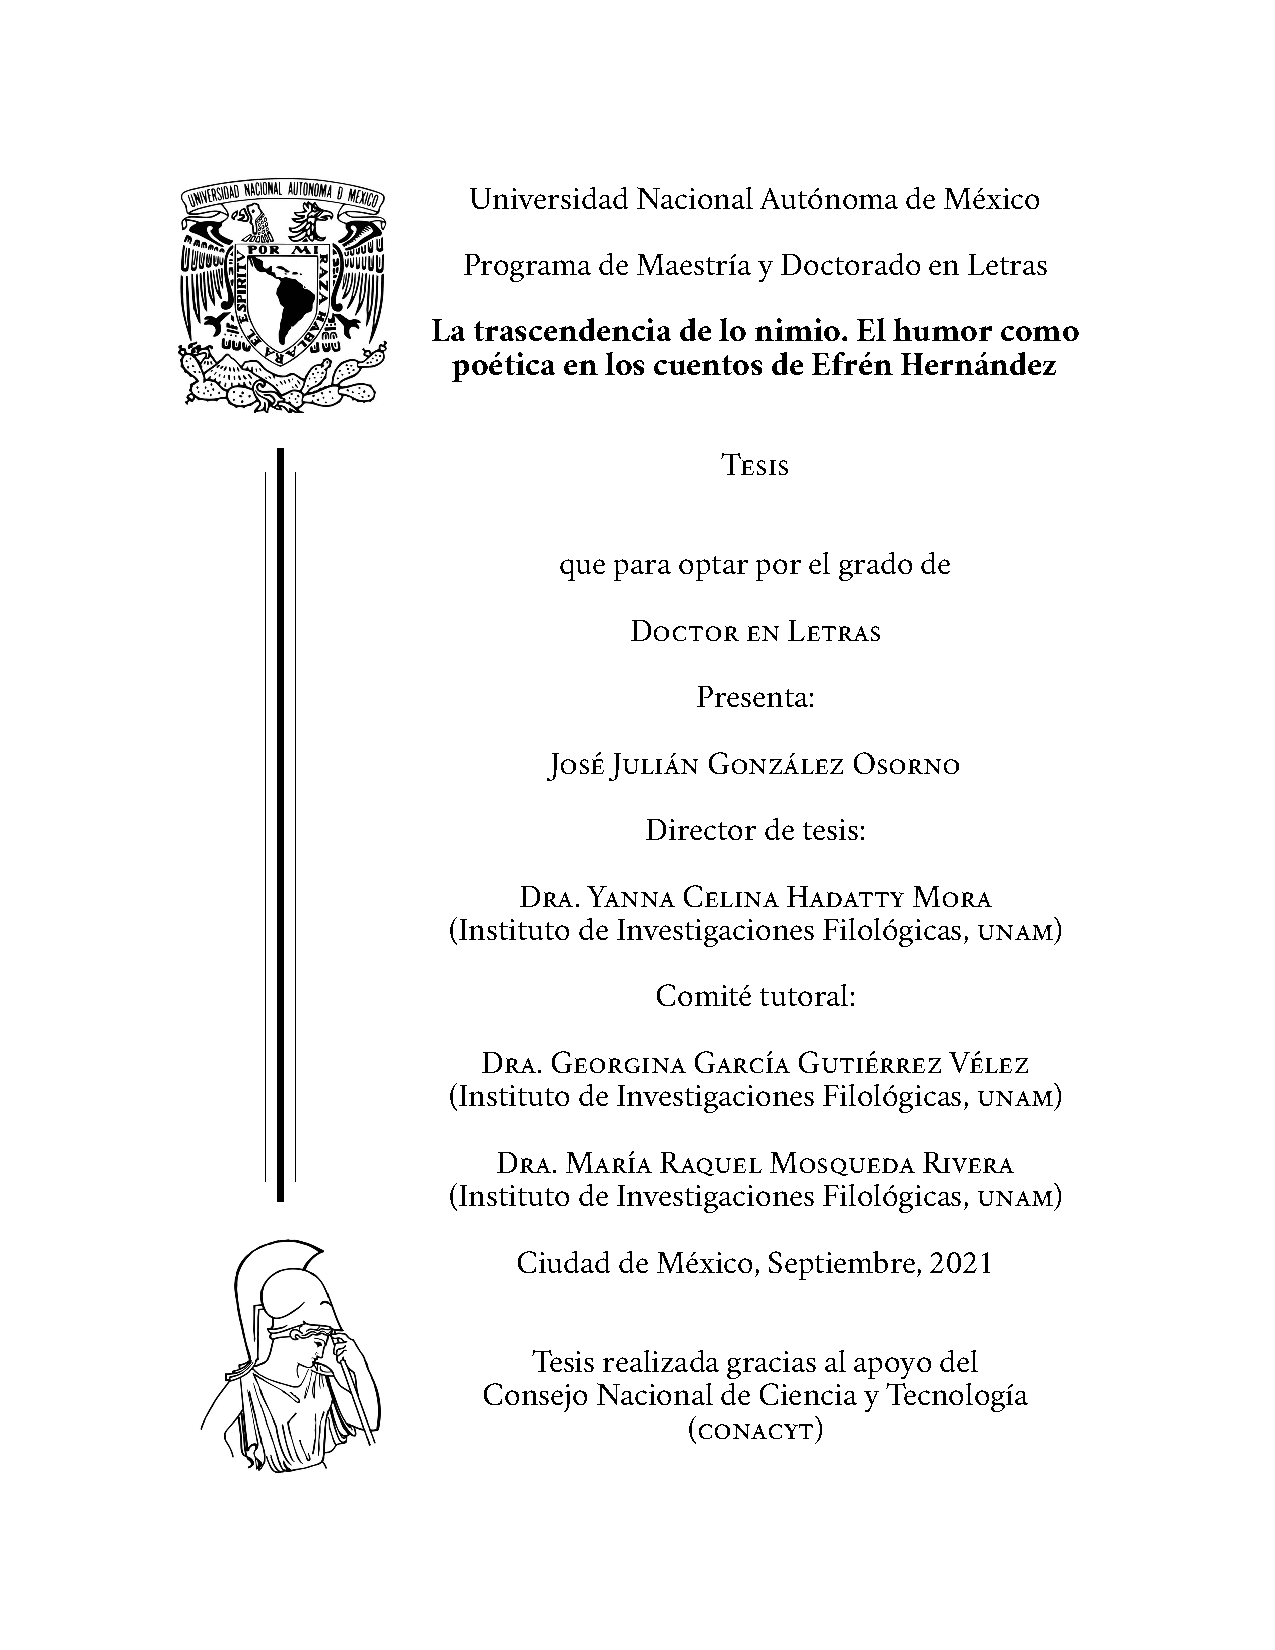
\includepdf[noautoscale]{Portada}
%\begin{center}
%
\includegraphics[width=3cm]{01} % 3cm para carta, 2cm para medio oficio
%\end{center}
%{\centering\biolinum
%Universidad Nacional Autónoma de México
%\vfill
%Programa de Maestría y Doctorado en Letras
%\vfill
%{\large\emph{La transcendencia de lo nimio. El humor como poética en los cuentos de Efrén Hernández}}
%\vfill
%\textsc{Tesis}
%\vfill
%que para optar por el grado de
%\vfill
%\textsc{Doctor en Letras}
%\vfill
%Presenta:
%\vfill
%\textsc{José Julián González Osorno}
%\vfill
%Director de tesis:
%\vfill
%\textsc{Dra. Yanna Celina Hadatty Mora} \\
%(Instituto de Investigaciones Filológicas, \textsc{unam})
%\vfill
%Comité tutoral:
%\vfill
%\textsc{Dra. Georgina García Gutiérrez Vélez} \\
%(Instituto de Investigaciones Filológicas, \textsc{unam})
%\vfill
%\textsc{Dra. María Raquel Mosqueda Rivera} \\
%(Instituto de Investigaciones Filológicas, \textsc{unam})
%\begin{center}
%Ciudad de México, \hl{Septiembre}, 2021
%\end{center}
%}
% PÁGINA EN BLANCO
\newpage
\pagestyle{empty}
\null\vfill
% GITHUB HOSTING
{
\noindent\footnotesize Esta tesis está disponible en \faGithub \\

\noindent\footnotesize\textbf{\url{https://tuxkernel.github.io/julian/}}
}
% DEDICATORIA
\newpage
\pagestyle{empty}
\pdfbookmark{Dedicatoria}{Dedicatoria}
\hspace*{0pt}
\vspace*{42pt}
% \ding{166} <--- Hoja (pifont)
\begin{flushright}
\textit{Para Mara y Elías} \ding{166}
\end{flushright}
% PÁGINA EN BLANCO
\newpage
\pagestyle{empty}
\null\vfill
% AGRADECIMIENTOS
\chapter*{Agradecimientos}\label{ch:agradecimientos}
\thispagestyle{empty}
\pagestyle{fancy}
\fancyhf{} % Remueve encabezados y pies previos. Necesario sí o sí.
\fancyhead[RE,LO]{\small\sc agradecimientos} % \small para carta; \footnotesize oficio.
%\fancyhead[]
\fancyhead[LE,RO]{\textlf{\thepage}}
\renewcommand{\headrulewidth}{0pt}
\pagenumbering{arabic}
\setcounter{page}{5}
\addcontentsline{toc}{chapter}{Agradecimientos}
Un trabajo de investigación es fruto de diversos apoyos, complicidades, gustos y voluntades. Aunque la responsabilidad de esta tesis es totalmente mía, deseo expresar mi gratitud a Alejandro Toledo, por su amistad y por facilitarme hace algunos años inéditos de Efrén Hernández que ahora integran el segundo volumen de las \emph{Obras completas} del autor guanajuatense (México, Fondo de Cultura Económica, 2012); colaborar con él en esta edición fue de total aprendizaje.

Gracias a la doctora Lourdes Franco Bagnouls, porque sin su lectura y estímulo este trabajo, en su primera parte, no hubiera sido posible. Mucho le debo asimismo a la Dra.\,Martha Elena Munguía Zatarain, admirada maestra de la Universidad Veracruzana; sus observaciones y textos fundamentales sobre la risa en la literatura mexicana fueron vitales para este análisis. Gracias también al Dr.\,Sergio López Mena, quien con su lectura inteligente y generosa hizo que este trabajo mejorara sustancialmente; al Dr.\,Juan Coronado, por sus aportaciones y recomendaciones.

Mi profundo agradecimiento a las doctoras integrantes de mi Comité tutor, Dra.\,Georgina García Gutiérrez y Dra.\,Raquel Mosqueda Rivera, cotutoras, y a la Dra.\,Yanna Hadatty Mora, tutora. Sin su atenta lectura, observaciones críticas y apoyo sin reservas este trabajo no hubiera sido posible. Gracias, en especial, a la Dra.\,Hadatty, por aceptar dirigirme.

Gracias a Víctor González Osorno e Iván González Osorno, mis hermanos, por su apoyo de siempre; a Dahlia Antonio Romero, por su lectura atenta y sugerencias; a Noel Merino Hernández, mi amigo de siempre, por maquetar este texto y por enseñarme, entre café y té, algunos principios sobre tipografía y diseño editorial.

Por último, expreso mi gratitud eterna a la Universidad Nacional Autónoma de México (\textsc{unam}). Ser un alumno de esta institución es un orgullo y una alta responsabilidad; al Consejo Nacional de Ciencia y Tecnología (\textsc{conacyt}), por brindarme una beca para realizar este trabajo durante el periodo 2007-2011; y, finalmente, agradezco a los investigadores y profesores de la maestría en Literatura Mexicana de la Universidad Veracruzana (\textsc{uv}), quienes, con sus enseñanzas, hicieron posible que yo fuese un alumno de esta prestigiosa universidad, la \textsc{unam}.
% CONTENIDO
% Remueve los puntos en los índices
\makeatletter
\renewcommand\@dotsep{200}
\makeatother
\renewcommand{\contentsname}{Contenidos}
\tableofcontents
\addcontentsline{toc}{chapter}{Contenidos}
\thispagestyle{empty}
\pagestyle{fancy}
\fancyhf{} % Remueve los encabezados y pies previos. Necesario sí o sí.
\fancyhead[RE,LO]{\small\sc contenidos}
\fancyhead[RO,LE]{\thepage}
\fancyfoot{}
\renewcommand{\headrulewidth}{0pt}
\pagenumbering{arabic}
\setcounter{page}{7}
% PÁGINA EN BLANCO
\newpage
\pagestyle{empty}
\null\vfill
% EPÍGRAFES
\newpage
\pagestyle{empty}
\vspace*{42pt}
\begin{flushright}
\begin{minipage}{7.5cm} % 7.5cm para carta; 6cm para medio oficio.
\emph{Efrén Hernández era capaz de orientar rumbos literarios, encender palabras y pensamientos.}
\begin{flushright}
\textsc{Dolores Castro}
\end{flushright}
\vspace*{28pt}
\emph{Efrén parecía un pajarito, pero con unas enormes tijeras de podar me fue quitando toda la hojarasca.}
\begin{flushright}
\textsc{Juan Rulfo}
\end{flushright}
\end{minipage}
\end{flushright}
% INTRODUCCIÓN
\chapter*{Introducción. Aproximación a <<Tachas>>}\label{ch:introduccion-aproximacion-a-tachas}
\thispagestyle{empty}
\pagestyle{fancy}
\fancyhf{} % Remueve los encabezados y pies previos. Necesario sí o sí.
\fancyhead[RE]{\small\sc el humor como poética en los cuentos de efrén hernández} % \small para carta, \footnotesize para medio oficio.
\fancyhead[LO]{\small\sc introducción. aproximación a <<tachas>>}
\fancyhead[RO,LE]{\textlf{\thepage}}
\renewcommand{\headrulewidth}{0pt}
\pagenumbering{arabic}
\setcounter{page}{11}
\addcontentsline{toc}{chapter}{Introducción. Aproximación a <<Tachas>>}
\section*{Semblanza del autor y contexto sociocultural}\label{sec:semblanza-del-autor-y-contexto-sociocultural}
\addcontentsline{toc}{section}{Semblanza del autor y contexto sociocultural}
Como cualquier lector inicial de Efrén Hernández, lo primero que conocí de él fue ese breve relato que aparece en diversas antologías del cuento mexicano del siglo \textsc{xx}: <<Tachas>> (1928). Muchos dicen que, al terminar de leerlo, se tiene la sensación de que se trata de un cuento pleno de inocencia y de fino humor, melancólico. No fui la excepción. Tras leer todos sus cuentos reafirmé la idea de estar ante una obra que se reía sutilmente, <<sin aristas hirientes>> como decía Alí Chumacero, de sus personajes, de la trama, del lector, del narrador y aun del autor. Una narrativa, como \hl{(de)mostraré} en este trabajo, donde el humor es parte sustancial de su poética.

Sobre la vida de Efrén Hernández (León, Guanajuato, 1904-Ciudad de México, 1958) se sabe que a los veintiún años intentó estudiar Derecho en la Escuela Nacional de Jurisprudencia de la Ciudad de México, quizá tratando de emular a su padre, quien fue juez en la ciudad de Guanajuato. No obstante, solo cursó un año por parecerle <<vacío y sin meollo de sustancia verdadera lo que ahí se aprende>>.\footnote{Efrén Hernández, <<Ficha autobiográfica>>, en \emph{Obras} (pról. de Alí Chumacero; recopilación de textos de Miguel Capistrán, Alí Chumacero y Luis Mario Schneider; bibliografía de Luis Mario Schneider) México, Fondo de Cultura Económica, 1965, p. 3.} Creía que el conocimiento verdadero residía en <<los hombres de carne y hueso>>, en <<los libros buenos>> y en <<el mundo>>.\footnote{\emph{Idem.}}

Ese desdén hacia la vida universitaria se extendió, asimismo, a los padrinazgos políticos, académicos y culturales, y lo llevó a ejercer los más diversos trabajos para sobrevivir: vendió aretes de plástico, figuritas de yeso, lámparas, libros
y productos de la Compañía Nacional de Subsistencias Populares (\textsc{conasupo}); fue archivista y electricista. Antes de llegar a la Ciudad de México había sido aprendiz de botica, de zapatero, de platero y dependiente en una tienda de ropa. Durante su etapa en la Ciudad de México, recuerda su hija Valentina Hernández Ponzanelli, llegó incluso a hacerse pasar por <<Inspector de Salubridad>> en los puestos de comida solicitando una muestra para <<verificar>> su estado cuando el hambre arreciaba.\footnote{Esto me contó el poeta Fernando Rodríguez antes de darme la entrevista donde refería que, en ciertas temporadas, Efrén Hernández vendía aretes de plástico, figuritas de yeso y lámparas para sobrevivir. Esta entrevista (más la de Dolores Castro y Juan Bañuelos) puede consultarse en José Julián González Osorno, <<Efrén Hernández a tres voces>>, \emph{Texto Crítico, Nueva Época}, año \textsc{xii}, núm. 24, enero-junio, 2009, pp. \mbox{139-145}; también en Juan M. Berdeja y Julián Osorno, \emph{Mirar no es como ver. Ensayos críticos sobre la obra de Efrén Hernández}, México, Universidad Autónoma de Querétaro, 2018, pp. 209-217. \hl{Las citas están hechas todo un chilaquil. Revisar el aparato crítico con más calma.}} Sus dos empleos mejor pagados quizá fueron el de oficinista en la Secretaría de Educación Pública (\textsc{sep}), junto a Juan Rulfo, y como subdirector de la revista \emph{América}.

Efrén Hernández fue un atento lector de una amplia tradición literaria y filosófica, clásica y moderna.\footnote{Entre estos autores pueden citarse: Cervantes, Santa Teresa, San Juan de la Cruz, Fray Luis de León, Quevedo y Góngora; filósofos como Demócrito, Sócrates, Platón, Plotino, Pascal, Nietzsche y Heidegger. Además de Don Juan Manuel, Shakespeare, Giono, Gracián, Gómez de la Serna, Hamsun
y Faulkner; y textos como \emph{El Panchatantra} y \emph{Las mil y una noches}. Cfr. Marco Antonio Millán, \emph{La invención de sí mismo} (ed. de Daniel González Dueñas y Alejandro Toledo), México, Consejo Nacional para la Cultura y las Artes, 2009, pp. 75 y 81; <<Efrén Hernández a tres voces>>, art. cit.; Federico S.\,Inclán, <<Carta a un amigo ausente>>, \emph{América. Revista Antológica}, Época Nueva, núm. 73, septiembre-octubre, 1959, p. 15.} Aunque breve, su obra abarca cuento, poesía,\footnote{Sus poemas están contenidos en los libros \emph{Hora de horas} (1936) y \emph{Entre apagados muros} (1943).} teatro,\footnote{Sus obras de teatro son \emph{Adanijob (fragmento)} y \emph{Cederano}, rescatadas por Alejandro Toledo del archivo de Efrén Hernández y publicadas en el tomo \textsc{ii} de las \emph{Obras Completas} (2012).} novela,\footnote{Sus novelas son \emph{Cerrazón sobre Nicómaco. Ficción harto doliente} (1946), \emph{La paloma, el sótano y la torre} (1949), \emph{Abarca. Fragmento de novela} (1949) y \emph{Autos}, descubierta por Alejandro Toledo entre los papeles de Efrén Hernández y publicada en 2007 en el tomo \textsc{i} de las \emph{Obras Completas}.} crítica literaria\footnote{Los ensayos son los comentarios de Efrén acerca de obras de diversos autores, sobre todo
mexicanos, contemporáneos a él. La mayoría recopilados por primera vez por Franco en \emph{Bosquejos} (1995). \ding{43} \hyperref[bib:franco1995]{Fuentes consultadas}.} y dos guiones para cine, uno para la actriz María Douglas y otro para Cantinflas.\footnote{Alejandro Toledo, <<El guión [\emph{sic}] que Cantinflas no pudo filmar>>, \emph{El Universal}, 7 de agosto, 2011; \emph{Obras \textsc{ii}}, Fondo de Cultura Económica, México, 2012, p. 5. \emph{Videm} <<El ``Tachas'' [\emph{sic}] escribe un asunto para Cantinflas>>, \emph{Prensa Gráfica}. México, 21 de mayo, 1949; <<Cantinflas tiene a su alcance el argumentista que necesitaba>>,  \emph{Ovaciones}. México, 1 de febrero, 1950.} Considerados como obras de teatro en las \emph{Obras completas}, \emph{Casi sin rozar el mundo} (1956) fue escrito para María Douglas y \emph{Dichas y desdichas de Nicócles Méndez; tragiburledia cinematográfica} (1951) para Cantinflas, esta a petición de Andrés Serra Rojas ---entonces director del Banco Nacional Cinematográfico.

Se creía que \emph{Dichas y desdichas de Nicócles Méndez} había sido escrita junto con Dolores Castro, Rosario Castellanos y Marco Antonio Millán; de hecho, se publicó en la revista \emph{América} (núm. 65, abril, 1951) como obra colectiva. No obstante, Dolores Castro le aclaró después a Alejandro Toledo: <<la invitación a participar en ese proyecto fue un acto de generosidad con dos jóvenes ---ella y Rosario Castellanos--- que se iniciaban en el mundo de las letras y con Millán, que era su mejor amigo>>. El texto se puede acreditar <<casi enteramente a Efrén Hernández>>.\footnote{Toledo, loc. cit.} Y en efecto, quienes leyeron esta obra aseguraban que había nacido \emph{el verdadero guionista de Cantinflas}.
\section*{La revista \emph{América} y el descubrimiento de Juan Rulfo}\label{sec:La-revista-américa-y-el-descubrimiento-de-juan-rulfo}
\addcontentsline{toc}{section}{La revista \emph{América} y el descubrimiento de Juan Rulfo}
Efrén Hernández fue, asimismo, un editor generoso que descubrió e impulsó a otros escritores, como Juan Rulfo. De esto da fe su participación en la revista \emph{América}, a la que ayudó a consolidar dándole un enfoque más literario en su calidad de subdirector.\footnote{Cfr. Lourdes Franco Bagnouls, \emph{Bosquejos} (ed., pról., ns. e índices), México, Universidad Nacional Autónoma de México"/Instituto de Investigaciones Filológicas"/Centro de Estudios Literarios, 1995 [Nueva biblioteca mexicana].} Fundada por miembros de las Juventudes Socialistas Unificadas de México (los poetas Roberto Guzmán Araujo, Manuel Lerín y el ensayista Agustín Rodríguez Ochoa) y por miembros de la Juventud Socialista Española,\footnote{Cfr. Elvira Acuña González, \emph{Índices de \emph{América}. Revista Antológica}, México, Universidad Iberoamericana, 2000, pp. 5-10 [Tesis de Licenciatura].} en sus primeros números Alfonso Reyes figuró como miembro de su comité editorial. Efrén Hernández fue invitado en 1942 por Marco Antonio Millán, el entonces Director de la revista, para desempeñarse como editor. Al principio se negó porque le parecía un medio muy político. Finalmente aceptó. Sus primeras participaciones las rubricó como <<Till Ealing>>; meses después firmó ya con su nombre. Como subdirector, su presencia fue vital para promover a jóvenes escritores de México.\footnote{Millán, \emph{op. cit.}, pp. 72-73.}

\emph{América} jugó un papel importante en la vida cultural de México de 1940 a
1969, comparable quizá al que desempeñaron, también en la primera mitad del siglo
\textsc{xx}, \emph{Taller}, \emph{Contemporáneos}, \emph{Examen}, \emph{Letras de México}, \emph{El Hijo Pródigo}, \emph{Rueca}, \emph{Pan}, \emph{Dintel}, \emph{Espiral}, \emph{Fuensanta}, \emph{Metáfora}, \emph{Tiras de Colores} o \emph{Estaciones}. Su criterio editorial de apoyar a <<gente de letras nueva, valiosa, desconocida o subestimada>>\footnote{Rosario Castellanos recuerda de la participación de Efrén Hernández en la revista: <<Durante el tiempo que tuvo a su cargo la dirección de \emph{América} abrió las puertas de par en par a quienes, sin más carta de recomendación que sus manuscritos, se acercaban en busca de un espacio en el cual divulgar [\emph{sic}] la buena nueva de sus creaciones literarias>>. Acuña González, \emph{op. cit.}, p. 20. \emph{Videm} Rosario Castellanos, \emph{Obras \textsc{ii}. Poesía, teatro y ensayo}, Fondo de Cultura Económica, México, 1998, p. 474.} fue un impulso en la difusión de la obra de, entonces, jóvenes escritores como Juan Rulfo, Jaime Sabines, Emilio Carballido, Edmundo Valadés, Rosario Castellanos, Juan José Arreola y Dolores Castro, entre otros. Sus miles de páginas, durante este periodo, mostraron parte de la poesía, la novela, el cuento, el teatro, el ensayo y la crítica de México y otros países latinoamericanos.

Sobre la importancia de esta revista en la promoción de jóvenes escritores, en 1993 Sergio López Mena había señalado el impulso que esta publicación dio a las primeras creaciones de Rulfo y de otros importantes escritores, y el papel destacado que tuvo en ello Efrén Hernández.\footnote{Cfr. Sergio López Mena, \emph{Los caminos de la creación en Juan Rulfo}. México, Universidad Nacional Autónoma de México, 1993, pp. 59-71.} Algunos de estos escritores luego le expresarían su agradecimiento.

Rosario Castellanos, por ejemplo, le decía a Hernández en una carta de 1942, con timidez: <<siento por ustedes [Millán y él] una gratitud muy grande. Han sido tan cordiales, tan amables con nuestros balbuceos. Y recordando que usted es tan bueno y tan sencillo y sabiendo que yo jamás le diría estas cosas personalmente, me atreví a escribírselas>>.\footnote{En carta fechada en Tehuacán, Puebla, el 25 de septiembre de 1948, Rosario Castellanos agradecía a Efrén Hernández el apoyo que él y Marco Antonio Millán le habían dado a ella y a Dolores Castro al publicar sus primeros escritos (\emph{Apuntes para una declaración de fe}, con nota introductoria de
Millán) en la revista \emph{América}, además comentaba acerca de sus lecturas y daba su opinión sobre el inicio de la novela \emph{Cerrazón sobre Nicómaco}. \emph{Videm} Samuel Gordon y Fernando Rodríguez (eds.), <<Cartas de Rosario Castellanos a Efrén Hernández>>, \emph{Literatura mexicana \textsc{vii}} (1), 1996, pp. 187-188.}

Juan Rulfo comentó de él:
\begin{quoting}
en el archivo de Migración nada se movía porque a nadie le interesaba estar ahí. Con cada cambio de gabinete los corrían a todos, menos a los del archivo del cual ni se acordaban, y en ese departamento donde no sucedía nada nos fuimos a meter Jorge Ferretis y yo, a la sombra de Efrén Hernández \xout{Hernández}. No queríamos que nos viera nadie, para así dedicarnos a nuestras cosas>>.\footnote{Se ha comentado que Rulfo conoció a Efrén Hernández en 1935 en la Secretaría de Educación Pública o, quizá, en 1937, en Gobernación (Archivo de Migración), donde Hernández fungía como <<jefe>>; véase al respecto la entrevista de Elena Poniatowska a Juan Rulfo en Roberto García Bonilla, \emph{Un tiempo suspendido. Cronología de la vida y la obra de Juan Rulfo}. México, Consejo Nacional para la Cultura y las Artes, 2008, p. 92.}
\end{quoting}
Ahí Hernández descubrió que Rulfo escribía a escondidas y luego lo destruía. Intrigado, le solicitó que le mostrara sus cuentos y quedó asombrado. Se dice que
Hernández ayudó a pulir ciertos aspectos técnicos de la narrativa rulfiana, lo cual es difícil ahora saber; lo cierto es que Juan Rulfo reconoció en él a un maestro: <<a él le debo todo>>, dijo en una conferencia.\footnote{\emph{Videm} \emph{Cerrazón sobre Efrén Hernández (documental harto doliente)}, 2016, Canal 22"/Consejo Nacional para la Cultura y las Artes. Dirección: Eduardo González Ibarra. Producción: Enrique Quintero-Mármol.}

En la nota previa a <<La cuesta de las comadres>> (\emph{América}, 1948), Hernández
decía del descubrimiento de Rulfo, cito en extenso para apreciar mejor la
participación de Hernández en el rescate de este texto:
\begin{quoting}
Causa, a un tiempo, de mi más persistente desconcierto y mi mayor confianza, es la manera de rigor, la rigurosísima y tremenda aspiración, el ansia de superación artística de este nato escritor. Cosas que en buena ley son de envidiarse, él, por hallarlas ruines, ha venido rompiéndolas, tirándolas, deshaciéndose de ellas, ¡para volver a hacerlas!

Nadie supiera nada acerca de sus inéditos empeños, si yo no, un día, pienso que por ventura, adivinara en su traza externa algo que lo delataba; y no lo instara hasta con terquedad, primero, a que me confesase su vocación, enseguida a que me mostrara sus trabajos y, a la postre, a no seguir destruyendo.

Sin mí, lo apunto con satisfacción, <<La Cuesta de las Comadres>>, habría ido a parar al cesto [...].\footnote{Presentación a Juan Rulfo, <<La cuesta de las comadres>>, \emph{América}. México, 29 de febrero, 1948, núm. 55, pp. 31-38.}
\end{quoting}
Este impulso a Rulfo ha sido comparado incluso con el papel que desempeñó Max
Brod con la obra de Kafka.\footnote{Tal como Max Brod hizo con Kafka, apunta Nuria Amat, Hernández rescató a Rulfo del silencio, una generosidad con la palabra de otros escritores que parece hasta insólita en el ámbito literario: <<Lo que hizo en realidad Efrén fue potenciar el estilo personalísimo de su admirado amigo, limpiando
ripios, limando retóricas, librándolo de verbosidad y barroquismo y contribuyendo como nadie a un gran salto en la carrera de escritor de Rulfo>>. Nuria Amat, \emph{Juan Rulfo, el arte del silencio}, Barcelona, Ediciones Omega, 2003, p. 101 [Vidas Literarias].} En todo caso, Hernández fue para Rulfo, recordaba
Arreola, \emph{un alma necesaria y oportuna}.\footnote{Entrevista de Elena Poniatowska \emph{apud} García Bonilla, \emph{op. cit.}, p. 113.}

Por amistad y quizá en gratitud, Rulfo dio a Hernández para \emph{América} siete de
los diecisiete relatos que luego integrarían \emph{El Llano en llamas}: <<Nos han dado la tierra>> (agosto, 1945), <<Macario>> (1946), <<Es que somos muy pobres>> (agosto, 1947), <<La cuesta de las comadres>> (febrero, 1948), <<Talpa>> (enero, 1950), <<El Llano en llamas>> (diciembre, 1950) y <<Diles que no me maten>> (agosto, 1951).\footnote{Además de colaborador de la revista, Rulfo fue parte del comité directivo. Marco Antonio Millán comentó sobre la publicación paulatina de los cuentos de Rulfo en \emph{América}: <<Juan crecía en tanto le publicábamos poco a poco todo \emph{El Llano en llamas}>>. Millán \emph{apud} López Mena, \emph{op. cit.}, p. 67.}

Cabe anotar que dos de estos cuentos, <<Nos han dado la tierra>> y <<Macario>>, no fueron publicados inicialmente en \emph{América}, pues aparecieron por primera vez en \emph{Pan. Revista de Literatura}, coordinada por Juan José Arreola y Antonio Alatorre. No obstante, \emph{América} albergó estos siete cuentos antes de que aparecieran en el volumen \emph{El Llano en Llamas}, más el relato <<La vida no es muy seria en sus cosas>> (junio, 1945), que no fue incluido en dicho volumen.\footnote{Los cuentos de Rulfo publicados por primera vez en \emph{Pan} son: <<Nos han dado la tierra>>, núm. 2, julio, 1945, pp. 1-3 y <<Macario>>, núm. 6, noviembre, 1945, pp. 1-3. Los publicados por primera vez en \emph{América}: <<La vida no es muy seria en sus cosas>>, núm. 40, 30 de junio, 1945, pp. 35-36; <<Es que somos muy pobres>>, núm. 54, 30 de agosto, 1947, pp. 24-29; <<La Cuesta de las Comadres>>, núm. 55, 29 de febrero, 1948, pp. 31-38; <<Talpa>>, núm. 62, 29 de febrero, 1948, pp. 79-87; <<El Llano en llamas>>, núm. 64, diciembre, 1950, pp. 66-85; y <<Diles que no me maten>>, núm. 66, agosto, 1951, pp. 125-130. Cfr. García Bonilla, \emph{op. cit.}, pp. 411-412 y Acuña, \emph{op. cit.}, pp. 174-175.} Así, con el impulso de estas dos revistas, se iba perfilando y difundiendo, paulatinamente, el magistral libro de Rulfo antes de salir en su primera edición de 1953. Esto fue motivo de enemistad entre Rulfo y Marco Antonio Millán, Director de \emph{América}, dado que Rulfo había insinuado la posibilidad de que sus cuentos se publicaran todos, por primera vez, en la revista; finalmente, como se sabe, aparecieron bajo el sello del Fondo de Cultura Económica, en la colección Lecturas Mexicanas.
\section*{Rasgos generales de su narrativa}\label{sec:rasgos-generales-de-su-narrativa}
\addcontentsline{toc}{section}{Rasgos generales de su narrativa}
Efrén Hernández publicó sus cuentos entre 1928 y 1941, cuando la narrativa mexicana en boga tenía como tema central, o como uno de sus ejes principales, la Revolución Mexicana. Sus personajes, anónimos, marginales, distraídos, son soñadores y con frecuencia se demoran en algún circunloquio. Fundada en el humor, esta narrativa es ingenua, grave y disparatada a veces, una pluralidad de voces conversacionales que dialogan con ellas mismas, con el autor y con el lector.

Los temas que los ocupan son inocentes a simple vista: un clavito que flota en el aire y un escritor que intenta amarrar el tiempo para escribir una historia jamás
leída; una Santa Teresa con vida en un cuadro que convive con ratoncitos parlanchines y reflexivos; un pájaro pensante y refunfuñón, un estudiante distraído; un paralítico ansioso de moverse como los árboles; tomates adorados como santos; palabras que caminan, duermen y sueñan... Tras ellos, Hernández plantea, como
sin querer, asuntos que dejan perplejos a quienes acompañan su escritura.

Son personajes y temas, evidentemente, alejados de la estética de la Revolución Mexicana y de la prosa indigenista de principios del siglo \textsc{xx}; distantes
también de la narrativa de Contemporáneos, influida por la vanguardia europea que exploraba poéticamente al sujeto y postergaba la narración. Hay en la narrativa de Hernández, de manera intertextual y como proyección artística, cierto parentesco o afiliación a una tradición visible en obras como \emph{Don Quijote de la Mancha}, donde lo cotidiano, lo pequeño y lo absurdo son algo, al mismo tiempo, maravilloso y
trascendente.

De su escritura se ha dicho que es vanguardista. Podría pensarse en cierta similitud con este movimiento artístico, como comentaré en el primer capítulo, no obstante, su literatura se nutría del Siglo de Oro español (<<el mejor momento de mi propio y nativo idioma>>, decía Hernández), antes que en la de su siglo.\footnote{En el prólogo que escribe para \emph{Liras de amor y muerte}, de Roberto Guzmán Araujo, Hernández criticó mordazmente al estridentismo, al surrealismo (cuyos productos eran <<abortos prematuros>>), al dadaísmo (incapaz de quitarse su <<tartamudez>>), al simbolismo y al academismo. Para él, un escritor debía tener como directrices la originalidad, la sinceridad, la claridad, la sencillez y, sobre todo, debía beber de la tradición literaria propia y no de las corrientes de moda. \emph{Videm} Efrén Hernández, <<Sobre lo humano en la poesía>> y <<Del surrealismo>> en Franco Bagnouls, \emph{op. cit.}, pp. 33-39; 175-176.} Si compartía con el surrealismo, por ejemplo, que la imaginación era fundamental en la actividad artística, como Bretón asentaba en el primer manifiesto surrealista de 1924,\footnote{Cfr. André Breton, \emph{Manifiestos del surrealismo}, Argentina, Terramar, 2006.} o que la poesía era una forma de vida, se distanciaba de él porque no apelaba a un automatismo psíquico en la creación artística ni a un distanciamiento de lo social, tampoco pretendió expresar <<el funcionamiento real del pensamiento>>\footnote{\emph{Ibid}., p. 31.} o explorar otros experimentos vanguardistas. La narrativa de Hernández parece nutrirse de una concepción de la literatura donde esta es un referente por sí misma; para él toda obra tenía como fundamento lo humano, así, para desarrollar su poética ficcional, estuvo atento a su realidad y a las voces de su tradición literaria.

De tal modo, ajeno tanto de la narrativa del \textsc{xx} que transfiguró la historia en tema literario como de la de los Contemporáneos, Hernández creó personajes soñadores, distraídos por excelencia, divagadores, pobres; algunos de ellos escritores marginales que se enredan en circunloquios y se lamentan porque el cauce de su escritura se desborda, a menudo, entre las páginas de algún cuento. Hechos de presente, sus pensamientos y diálogos ocurren en el instante. Su ser y su transcurrir están despojados de la gravedad de la historia. Así, para ellos, la adoración de unos tomates puede ser más trascendente que el asesinato del presidente Álvaro Obregón, como se advierte en <<Unos cuantos tomates en una repisita>>.\footnote{Las excepciones serían \emph{Abarca} y, en menor grado, \emph{La paloma, el sótano y la torre}, novelas que no son objeto de estudio en este análisis. \emph{Abarca (Fragmento de novela)} trata de la lucha del revolucionario Teodoro Abarca contra los federales y está ambientada en el periodo de la Revolución mexicana; fue publicada como <<Abarca (Fragmento de una novela inédita)>> en \emph{América}, núm. 59, febrero, 1949, y, póstumamente, en las \emph{Obras} de 1965. Por otra parte, \emph{La paloma, el sótano y la torre} (1949), aunque su marco es la Revolución mexicana, la lucha civil no constituye su núcleo narrativo sino el triángulo amoroso entre sus principales personajes: Lina, Fulán y Catito.

En la década en que se publicaron las novelas de Efrén Hernández también hay narraciones que se alejan del canon revolucionario, pero que siguen teniendo un claro matiz realista. Entre estas pueden citarse: \emph{Los muros de agua} (1941) de José Revueltas; \emph{La barriada} (1948) de Benigno Corona Rojas; \emph{El sol sale para todos} (1948) de Felipe García Arroyo; \emph{Cabello de elote} (1949) de Mauricio Magdaleno; \emph{Sendas perdidas} (1949) de Mariano Azuela; \emph{La maestrita} (1949) de María Luisa Ocampo; \emph{Río humano} (1949) de Rogelio Barriga Rivas; y \emph{Ojo de agua} (1949) de Rubén Salazar Mallén. Entre los volúmenes de cuentos que ya no tratan el tema revolucionario están \emph{Cinco horas sin corazón} (1940) de Bernardo Ortiz de Montellano; \emph{La noche} (1943) de Francisco Tario y \emph{Varia invención} (1949) de Juan José Arreola.}
\section*{La \hl{risa} como poética. Propuesta de lectura}\label{sec:la-risa-como-poetica-propuesta-de-lectura}\nota{¿La risa o el humor? ¡Ummta madre!}
\addcontentsline{toc}{section}{La risa como poética. Propuesta de lectura}

Este trabajo busca \hl{(de)mostrar} que esa interrogante inicial surgida después de leer <<Tachas>> apuntaba en realidad por la unidad y el sentido artístico de la narrativa de Efrén Hernández; una interrogante que podemos empezar a responder mediante el estudio de las formas y tonos con que se manifiesta el humor en sus cuentos, visto este no como recurso retórico u ornato estético, sino, como mencioné, poética narrativa.

Para tal propósito, considero, fundamentalmente, el siguiente corpus de estudio: <<Tachas>> (1928) y los cuentos incluidos en \emph{El señor de palo} (1932): <<Santa Teresa>>, <<Un escritor muy bien agradecido>>,\footnote{En la edición de \emph{El señor de palo} (1932) y en la de 1956, \emph{Sus mejores cuentos}, publicada por editorial Novaro, este cuento aparece con el título <<Un gran escritor muy bien agradecido>>; en cambio, en las \emph{Obras} de 1965 del Fondo de Cultura Económica y en la más reciente, \emph{Obras completas \textsc{i}}, de 2007, se titula <<Un escritor muy bien agradecido>>. La variante, <<escritor>> en lugar de <<gran escritor>>, no afecta el sentido del cuento, aunque al leerlo es evidente el guiño irónico del autor al usar dicho adjetivo.} <<El señor de palo>>, <<Un clavito en el aire>>; así como los relatos de \emph{Cuentos} (1941), volumen que sumaba a <<Tachas>> y a los cuentos de \emph{El señor de palo}, <<Incompañía>>, <<Sobre causas de títeres>>, <<Unos cuantos tomates en una repisita>> y <<Una historia sin brillo>>. También los cuatro contenidos en \emph{Obras} (1965): <<Don Juan de las Pitas habla de la humildad>>, <<Toñito entre nosotros (estampa)>>, <<Trabajos de amor perdidos>>\footnote{El título del cuento alude a una de las primeras comedias de Shakespeare: \emph{Love's labours lost}, aunque no hay punto de comparación entre una historia y otra. Hernández publicó <<Trabajos de amor perdidos>> por primera vez en julio de 1941 y, por última, en 1952. En 1941 apareció con el subtítulo <<fragmento de novela>> en \emph{Letras de México}; en junio de 1942 con el título <<A rastras por el suelo>> y con el subtítulo <<fragmento de la novela Trabajos de amor perdidos>>. Esto hace suponer que Hernández estaba pensando en él como parte de una novela que no concluyó. El héroe de este cuento tiene un aire de familia con Catito, personaje de \emph{La paloma, el sótano y la torre} (1949). En 1952 se fue publicado con el subtítulo de <<fragmento de un cuento corto>>. \emph{Videm} \hyperref[bib:hernandez1952]{Fuentes consultadas.}} y <<Carta tal vez de más>>.
\section*{Estructura capitular}\label{sec:estructura-capitular}
\addcontentsline{toc}{section}{Estructura capitular}
La tesis se integra por tres capítulos. En el primero analizo la recepción de la obra de Hernández entre sus contemporáneos y estudiosos posteriores; exploro lo que ha dicho la crítica sobre la posible filiación de su obra a la vanguardia literaria hispanoamericana y reviso las apreciaciones de varios autores respecto del humor en esta obra. Además estudio la irrupción de la vanguardia y su estrecha relación con una risa de ruptura que sacudió las estructuras del cuento, lo cual le imprimió una transformación al género, incluso en Latinoamérica, en la que se aprecia claramente ese <<escribir contra la literatura>> que Rafael Lemus vio en Efrén Hernández.\footnote{Rafael Lemus, <<Informe>>, en Alejandro Toledo (comp.), \emph{Dos escritores secretos. Ensayos sobre Efrén Hernández y Francisco Tario}, México, Consejo Nacional para la Cultura y las Artes"/Fondo Editorial Tierra Adentro, 2006, pp. 117-118.}

En el segundo analizo cómo la perspectiva narrativa de un hombre interior se enlaza al humor y a las constantes digresiones de sus narradores. Este hombre interior, el héroe que suele protagonizar ---y, la mayoría de las veces, narrar---, asume la investidura de algunas figuras clásicas de la risa como el distraído, el niño o el ingenuo, y el paria o marginado (una de cuyas representaciones es el escritor fracasado), variaciones estas del tonto, la figura de la risa por excelencia, como
señaló Mijaíl Bajtín en su estudio sobre Rabelais,\footnote{Mijaíl Bajtín, \emph{La cultura popular en la Edad Media y en el Renacimiento. El contexto de Fran"cois Rabelais} (trad. de Julio Forcat y César Conroy), España, Alianza Editorial, 1987.} y profundizó Luis Beltrán en \emph{Anatomía de la risa}.

Finalmente, en el tercero, exploro algunas formas que la risa adquiere en esta cuentística: la relación entre el humor y lo cómico; la intertextualidad con la literatura de la risa y textos clásicos como la Biblia, a menudo desde un punto de vista paródico y desacralizador; el absurdo; el tono conversacional y humorístico hacia el lector, metanarrativo, donde se advierte la plena conciencia de su condición literaria. Cabe señalar que una parte preliminar de este capítulo fue publicada en \emph{Mirar no es como ver. Ensayos críticos sobre la obra de Efrén Hernández} con el título de <<Diálogos intertextuales en la cuentística de Efrén Hernández>>.

En suma, en este trabajo se analiza el papel de la risa en la configuración de los cuentos de Efrén Hernández, la cual es fundamental en la visión del mundo desde la que se escribe, no como recurso retórico sino como poética ficcional, es decir, la forma y proyección artística como se relatan los cuentos, la manera en que se configura el discurso, las temáticas y personajes. A través de la risa el autor disuelve los grandes discursos (la historia, entre ellos), los trastoca, los subvierte, y configura una narrativa donde se privilegia lo nimio, lo intrascendente, lo cotidiano.
% PÁGINA EN BLANCO
\newpage
\pagestyle{empty}
\null\vfill
% EPIGRAFE
\newpage
\pagestyle{empty}
\vspace*{42pt}
\begin{flushright}
\begin{minipage}{7.5cm} % 7.5cm para carta; 6cm para medio oficio.
\emph{La pugna de Efrén Hernández no es contra la literatura mexicana sino contra la literatura. Contra la trama. Contra el sentido. Contra el lenguaje. Contra todo
aquello que impide decir la vida amorfa.}
\begin{flushright}
\textsc{Rafael Lemus}
\end{flushright}
\end{minipage}
\end{flushright}
% CAPÍTULO 1
\chapter{Risa, vanguardia y cuento hispanoamericano}\label{ch:risa-vanguardia-y-cuento-hispanoamericano}
\backgroundsetup{
color=black,
scale=8,
hshift=26,
vshift=28,
angle=0,
opacity=.4,
contents=1
}
\BgThispage
\thispagestyle{empty}
\pagestyle{fancy}
\fancyhf{} % Remueve los encabezados y pies previos. Necesario sí o sí.
\fancyhead[RE]{\small\sc el humor como poética en los cuentos de efrén hernández} % \small para carta; \footnotesize para medio oficio.
\fancyhead[LO]{\small\sc i \textbullet\ risa, vanguardia y cuento hispanoamericano} % \small para carta; \footnotesize para medio oficio.
\fancyhead[RO,LE]{\textlf{\thepage}}
\renewcommand{\headrulewidth}{0pt}
\pagenumbering{arabic}
\setcounter{page}{25}
\section{Vanguardia y manifestación de la risa}\label{sec:vanguardia-y-manifestacion-de-la-risa}
La vanguardia, señala Saúl Yurkievich, <<instaura la ruptura de la tradición y la
tradición de la ruptura>>.\footnote{Saúl Yurkievich, <<Los avatares de la vanguardia>>. \emph{Revista iberoamericana}, 1982, vol. 48, no. 118, p. 351.} La razón es que los movimientos artísticos de la modernidad que componen la vanguardia (el cubismo, el futurismo, el expresionismo, el imaginismo, el dadaísmo, el ultraísmo y el surrealismo) resultan de una crisis y, en su afán de superarla, buscan romper radicalmente con el pasado. Por eso se trata de rupturas que aspiran a renovaciones profundas en el arte, a la transformación absoluta.\footnote{\emph{Idem}.}

Esa revolución se ancla, sobre todo, en un cuestionamiento de la racionalidad capitalista, de la ética y sentido del arte heredados de la sociedad decimonónica burguesa. Por eso la vanguardia acoge con alegría la ofensa al buen gusto burgués de los decadentistas y los simbolistas, y se orienta a la producción de nuevos símbolos culturales. La vanguardia, apunta Hugo Achugar, es
\begin{quoting}
un tipo de producción simbólica que disolvió definitivamente ciertas concepciones heredadas de la segura sociedad decimonónicamente burguesa, al proponer el relativismo de toda producción artística y filosófica como algo propio de una civilización que sabía o había aprendido la historicidad de todo lo construido por el hombre y su eventual caducidad. En cierto modo podría afirmarse que la vanguardia muestra la modificación, o mejor aún, la creación de un nuevo imaginario social.\footnote{Achugar \emph{apud} Hugo J.\,Verani (ed.), \emph{Narrativa vanguardista hispanoamericana}, México, Universidad Nacional Autónoma de México, 1996. p. 13.}
\end{quoting}
En este nuevo imaginario social, que toma fuerza principalmente en el París de finales del \textsc{xix}, el escenario hasta entonces reconocido como propio de la actividad artística cambia. Como asienta Bolívar Echeverría \xout{en <<De la academia a la bohemia y más allá>>}, la figura del artista se desplaza de los talleres de arte institucionales a cafés y cabarets, en los que, como puede advertirse en \emph{Baile en el Moulin de la Galette} de Renoir, <<la vida se libera de su compulsión productivista>>\footnote{Bolívar Echeverría, <<De la academia a la bohemia y más allá>>. \emph{Theoría. Revista del Colegio de Filosofía} 19 (2009), p. 51.} y se acerca al mundo de la fiesta, lo cual simboliza la vuelta del arte a su matriz premoderna. A partir de este desplazamiento, el arte de vanguardia deja atrás la \emph{mímesis de la realidad} y se resuelve en una \emph{mímesis festiva}, que es
\begin{quoting}
una mímesis de segundo grado, que no imita la realidad sino la desrealización festiva de la realidad; una mímesis que no retrata los objetos del mundo de la vida sino la transfiguración por la que ellos pasan cuando se encuentran incluidos en otra mímesis, aquella que la existencia festiva hace del momento extraordinario del modo de ser humano.\footnote{\emph{Ibid.}, p. 55.}
\end{quoting}
La fiesta es una interrupción del modo ordinario de la vida humana, y una de sus señas es la irrupción de un caos lúdico vinculado a la risa. Es como si en la fiesta <<el caos ---lo otro, humanizado o ``domesticado'' como la contraparte del cosmos humano--- hiciera un gesto de amenaza, fingiera hacer estallar esa humanización o ``domesticación'', destruirla (así sea, lúdicamente, para reconstruirla después)>>.\footnote{\emph{Ibid.}, p. 53.} En esta destrucción de la fiesta, la risa es la gran protagonista.

El mundo en que nacieron las vanguardias, el de los cafés y cabarets, no es el de la fiesta popular masiva, de épocas anteriores a la modernidad, como el carnaval medieval, pero conserva parte de su esencia y no se disuelve por completo en la privatización o el individualismo del tiempo de ocio.\footnote{Luis Beltrán anota que <<En Occidente, la fiesta semanal se ha convertido en el fin de semana, de momento de dos días. Y aún se le añaden los periodos de vacaciones. El resultado es la pérdida del sentido alegre de la fiesta y de la comunidad feliz. La fiesta deja de ser el tiempo de la alegría, de la risa, para convertirse en el tiempo del ocio, un tiempo sin actividad productiva, un tiempo para el aislamiento>>. Luis Beltrán Almería, \emph{Anatomía de la risa}, México, Ediciones Sin Nombre"/Consejo Nacional
de Ciencia y Tecnología"/ Universidad de Sonora, 2011, p. 19 [Relámpago la risa; coord. Martha Elena Munguía Zatarain].} La vida de los cafés y cabarets, pese a estar inscrita en el tiempo del ocio, es un cronotopo festivo en el que surge, aunque restringido, el ambiente de la fiesta universal, sobre todo a través de la ingesta de alcohol. Sus participantes, como los de la gran fiesta universal, también experimentan una liberación transitoria a través de la que acceden al <<reino utópico [...], de la libertad, de la igualdad y de la abundancia>>.\footnote{Bajtín, \emph{op. cit}., p. 15. \hl{Esta cita está mal. No se ha citado anteriormente a Bajtín en alguna de sus obras y, por lo tanto, no se puede poner \emph{op. cit.} Existe otro problema; en la bibliografía final hay tres obras de Bajtín. ¿A cuál de ellas se refiere esta cita? ¿1989? ¿1993? ¿2005? Julián, indicame a cuál de ellas se refiere.}}

En \emph{Historia de la risa y la burla}, Georges Minois comenta sobre ese ambiente a través de la figura del borrachín en los cafés franceses de fines del siglo \textsc{xix}: <<se revuelca en el lodo, apesta, vomita, escupe, orina, se pee. Su apestoso talante pertenece a la muy popular boga de la suciedad que amenizaba los cafés-concierto, o a los lectores del \emph{Journal des merdeux}>>.\footnote{\emph{Le Journal des merdeux} (trad. al esp. como \emph{El Diario de mierda}) fue una publicación finisecular de un único número editada en 1882 por Jules Jouy (1855-1897). George Minois, \emph{Historia de la risa y la burla: del Renacimiento a nuestros días}, México, Universidad Veracruzana"/Ficticia"/Consejo Nacional de Ciencia y Tecnología, 2018, p. 290.}

El borrachín es la encarnación del caos lúdico que surge en la fiesta, de ahí su fuerza nihilista, destructiva. ¿Podemos dudar de que el borrachín es imagen del
caos festivo, que, como señala Echeverría, es la pantomima de una amenaza que se dirige a la domesticación humana y finge destruirla?

En ese París finisecular que evoca Minois, el arte no solo estaba impulsado por la risa insensata y descabellada, también por un humor oscuro y desencantado representado por Georges Courteline (1859-1929). Ambos talantes, sin embargo, partían de un punto común enraizado en el espíritu de los tiempos: <<el sentimiento del sinsentido del universo y el carácter indeterminado, indecidible, de las cosas>>.\footnote{\emph{Ibid.}, p. 358.} En honor a este sentimiento es que <<entre la depresión y la fantasía, el hombre de fines de siglo flota, sin puntos de referencia, riéndose de todo y de nada [...]>>.\footnote{\emph{Ídem.}} Fue esta risa insensata, descabellada, oscura, hija del sinsentido, la que hizo del París de la Bella Época la capital de la risa y de la vanguardia, pues esta heredó de aquella
su fuerza nihilista, caótica y destructiva.

Son incontables las veces en que la ruptura de la tradición que instauró la vanguardia se dio a través de la risa, como podemos apreciar en <<Dadá manifiesto sobre el amor débil y el amor amargo>>, de Tristan Tzara (\mbox{1896-1963}), que es una suerte de irónicas instrucciones <<Para hacer un poema dadaísta>>, de una risa cuyo objetivo es la tradición y, en un giro de autoescarnecimiento, el mismo movimiento Dadá.\footnote{Tristan Tzara. \emph{Siete manifiestos Dadá}. México, Tusquets, 2013, p. 50.}
\section{¿Un escritor de vanguardia u original? Interpretaciones de sus relatos}\label{sec:un-escritor-de-vanguardia-u-original-interprestaciones-de-sus-relatos}
La narrativa de Efrén Hernández ha sido ligada a la vanguardia iberoamericana de los años veinte y principios de los treinta. Esta tesis fue sugerida por John Brushwood, para quien Hernández es un escritor moderno porque <<va desde los experimentos de la época vanguardista hasta la reafirmación de las mismas tendencias en la nueva novela>>.\footnote{John Brushwood, <<Efrén Hernández y la innovación narrativa>>, \emph{Nuevo Texto Crítico}, \textsc{i}, (1988), p. 93.}

En 1995 Franco Bagnouls señaló la aparente paradoja respecto de la pertenencia o no de Hernández a la vanguardia, al preguntarse en Bosquejos: <<¿por qué [Efrén Hernández] parece criticar en sus artículos ciertas formas de lo literario [vanguardistas] que se dan en la narrativa escrita por él?>>.\footnote{Franco, \emph{op. cit.}, p. 25. \hl{Esta cita también está mal. No se ha citado a Franco Bagnouls con anterioridad. Esta cita a qué obra obra corresponde de la bibliografía final. ¿1989? ¿1995? o ¿2008?}} La similitud entre la escritura de Hernández y las vanguardias, según Franco, puede entenderse a la luz de <<una nueva estética presidida por la ruptura con la realidad tangible e inmediata
en busca de nuevas formas de asociación>>.\footnote{\emph{Ibid.}, p. 26. \hl{La cita está mal. Mientras no sepa a que obra se refiere la cita anterior, no se puede continuar.}} En esta búsqueda, la exploración de los mecanismos del inconsciente era importante pero no determinante. Jairo Castillo\footnote{Jairo Francisco Castillo Díaz, \emph{Una aproximación a la cuentística de Efrén Hernández}. Universidad
Nacional Autónoma de México, México, 1996. [Tesis de licenciatura].} agrega que esta idea de literatura moderna se sustentaba en la plena autonomía del texto literario frente al autor.

También Hugo J.\,Verani (1996)\footnote{Verani incluye a Hernández, como representante de la vanguardia hispanoamericana, al lado de Roberto Artl, Macedonio Fernández, Oliverio Girondo, Pablo Palacio, Vicente Huidobro, Pablo Neruda, Martín Adán, César Vallejo, Felisberto Hernández, Julio Garmendia, Salvador Novo, Arqueles Vela y Gilberto Owen. El estudio-antología contiene <<Tachas>> como uno de los cuentos mexicanos representativos de esta estética. Hugo J.\,Verani (ed.), \emph{Narrativa vanguardista hispanoamericana}, Universidad Nacional Autónoma de México, México, 1996.} y Fernando Burgos (1997)\footnote{Burgos selecciona <<Un clavito en el aire>> como cuento representativo de Hernández de la estética vanguardista. Fernando Burgos (introd. y ns.), \emph{El cuento hispanoamericano en el siglo \textsc{xx}}, Madrid, Castalia, 1997.} consideraron a Efrén Hernández en sus antologías sobre narrativa vanguardista. Asimismo, las reflexiones de Yanna Hadatty (2003) no deben perderse de vista al intentar comprender dicha adscripción, porque hay en su obra temprana, señala Hadatty, ciertos elementos del dadaísmo, del surrealismo, del cubismo y del expresionismo.\footnote{Yanna Hadatty Mora, \emph{Autofagia y narración. Estrategias de representación en la narrativa
iberoamericana de vanguardia, 1922-1935}, Madrid, Iberoamericana"/Vervuet, 2003, pp. 96-97.} Críticos como Esperanza López Parada y Rafael Lemus afirman que Hernández
es un inclasificable, un \emph{outsider}, un marginal. Un novelista distinto entre los distintos, lo llama López Parada, por ser su escritura descentrada y rebasar los géneros.\footnote{Esperanza López Parada, \emph{Una mirada al sesgo. Literatura hispanoamericana desde los márgenes}. Madrid"/Frankfurt, Iberoamericana"/Vervuert, 1999, pp. 11-12.} Escritura que semeja el camino que traza la silla de ruedas de <<El señor de palo>>: no sigue la línea recta de la narrativa tradicional, pues, como una raíz o un rizoma, transita por líneas alternativas.\footnote{\emph{Ibid.}, p. 12.}

Por su parte, Rafael Lemus anota sobre la excentricidad de Efrén Hernández, vale la pena citarlo en extenso por su planteamiento:
\begin{quoting}
Se dice: es raro porque es secreto. Porque se opone al cauce principal, realista, de la literatura mexicana. Porque no es Juan Rulfo o Carlos Fuentes. Se repasa su obra ---una novela, dos docenas de relatos, una obra teatral, algunos poemas--- como para despacharla apresuradamente. Para decir: sí, es rara. Para apuntar: no, no es \emph{La sombra del caudillo} o \emph{La tumba}. Quien así procede ---así proceden casi todos--- no comprende lo esencial. Esto: la pugna de Efrén Hernández no es contra la literatura mexicana sino contra la literatura. Contra la trama. Contra el sentido. Contra el lenguaje. Contra todo aquello que impide decir la vida amorfa. Por eso hay que leerlo fuera de su contexto inmediato. Hay que decir: Efrén Hernández es mexicano, y otra cosa. Decir: es un autor mayor, a veces enorme, y leerlo al lado de otros autores mayores, a veces enormes. Leerlo, sobre todo, para entender el cómo. ¿Cómo se impide fijar? ¿Cómo pronuncian aquí y allá lo informe? Leerlo para descubrir un método. Una escritura de lo informe.\footnote{Lemus, \emph{op. cit.}, p. 43. \hl{Otra cita mal, pues no se ha citado anteriormente a Lemus. Ese es el pedo de quitar texto sin revisar nuevamente el aparato crítico. No va a quedar de otra que copiar la referencia de la bibliografía final y poner acá.}}
\end{quoting}
López Parada y Lemus coinciden en que Hernández no sigue el modelo mimético realista (aristotélico); su obra es propia de una literatura posmoderna: fragmentaria, digresiva, que niega la discursividad grandilocuente.

Lectores y críticos han visto en Efrén Hernández a un escritor autobiográfico, \emph{sui generis}, que rompe con las formas de narrar realistas, un escritor vanguardista, a pesar suyo, en cuya escritura la risa tiene un papel fundamental.
\section{Cuentistas hispanoamericanos de vanguardia}\label{sec:cuentistas-hispanoamericanos-de-vanguardia}
En su \emph{Antología crítica del cuento hispanoamericano del siglo \textsc{xx} (1920-1980)}, José Miguel Oviedo señala que la vanguardia en Hispanoamérica tiene un desarrollo <<autónomo, divergente y profundamente creador>>, en el que se involucran <<fuerzas propias que exceden, estética y cronológicamente, las propuestas originales de la vanguardia>>.\footnote{José Miguel Oviedo, \emph{Antología crítica del cuento hispanoamericano del siglo \textsc{xx} (1920- 1980). \textsc{i}. Fundadores e innovadores}, Madrid, Alianza Editorial, 2002, p. 13.} Un claro ejemplo es el creacionismo del poeta chileno Vicente Huidobro, cuyos presupuestos teóricos se asientan en el manifiesto \emph{Non serviam}, de 1914, y al que da una forma más acabada en 1916, poco antes de viajar a Europa. El caso del creacionismo permite lanzar la idea, señala Oviedo, de que <<la literatura de vanguardia no se desplaza en un solo sentido a través del Atlántico: es un vaivén; mejor aún: una red que se abre en múltiples direcciones interconectadas>>.\footnote{\em Idem.} Otro ejemplo es el del surrealismo, que si bien nace en Francia, se arraiga en Hispanoamérica con características, alcances y propuestas propias.

1914, año en que Huidobro dio lectura pública a \emph{Non serviam}, es considerado
por Jorge Schwartz el punto de arranque de las vanguardias en América Latina: <<Tanto por la actitud cuanto por los irreverentes postulados, \emph{Non serviam} representa el momento inaugural de las vanguardias del continente>>.\footnote{Jorge Schwartz, \emph{Las vanguardias latinoamericanas}, México, Fondo de Cultura Económica, 2006, p. 37.} Su declive en Hispanoamérica comienza a verse después de 1938, año del encuentro en México entre Diego Rivera, León Trotsky y André Breton y de la escritura conjunta del <<Manifiesto por un Arte Revolucionario Independiente>>, que según señala Schwartz, <<es importante por su influencia en la toma de posición política de los artistas europeos de vanguardia y sus repercusiones en América Latina>>,\footnote{\em Ibid. p. 40.} esto en relación a que reclamaba: <<La independencia del arte-por la revolución; La revolución-por la liberación definitiva del arte>>.\footnote{André Breton, León Trotski \emph{et al.}, \emph{Manifiesto por un arte revolucionario independiente}, México, Siglo \textsc{xxi}, 2019, p. 44.}

En el prólogo a \emph{Narrativa vanguardista hispanoamericana}, Hugo Achugar señala que los textos fundamentales de la vanguardia hispanoamericana pueden encontrarse en la segunda y tercera décadas del siglo \textsc{xx}.\footnote{Cuando el proceso de expansión del capitalismo se vería interrumpido por la Primera Guerra Mundial, 1914-1918, y el colapso de la Bolsa de Valores de Wall Street, 1929, que llevaría a una crisis económica mundial.} En la selección de Achugar y Verani se incluyen narraciones publicadas entre 1922 y 1932 por Roberto Artl y Macedonio Fernández (Argentina); Vicente Huidobro (Chile); Pablo Palacio (Ecuador); Martín Adán y César Vallejo (Perú); Efrén Hernández, Salvador Novo, Gilberto Owen y Arqueles Vela\footnote{Aunque Vela nació en Guatemala, la mayor parte de su vida se desarrolló en México.} (México); Felisberto Hernández (Uruguay) y Julio Garmendia (Venezuela). A decir de Achugar, estos autores <<propusieron un nuevo modo imaginario de entender y representar la vida cotidiana, tanto a nivel individual como social, a la vez que explotaron (¿explosionaron?) los fundamentos estéticos y artísticos heredados. Es decir, se apartaron de una concepción de una narrativa para proponer otra que negaba, hasta cierto punto, una tradición con larga vigencia>>.\footnote{Achugar \emph{apud} Verani, \emph{op. cit.}, p. 16.}

La lista de los cuentistas de vanguardia se enriquece con las incorporaciones que hace Fernando Burgos a \emph{El cuento hispanoamericano en el siglo \textsc{xx}}: el guatemalteco Rafael Arévalo Martínez; los chilenos María Luisa Bombal, Juan Emar y Héctor Barreto; el argentino Ricardo Güiraldes y el mexicano Julio Torri.\footnote{Cfr. Burgos, \emph{op. cit.}, p. 15.} En \emph{Voces recobradas. Narrativa mexicana fuera del canon (1925-1950)}, Lourdes Franco Bagnouls agrega a José Martínez Sotomayor, María Ramona Rey, Alberto Quintero Álvarez, César Garizurieta, Luis G. Basurto, Solón de Mel\footnote{El verdadero nombre de Solón de Mel era Guillermo de Luzuriaga y Bribiesca (Ciudad de México, 1895-1959). Fundó y dirigió revistas como \emph{El trovador}, \emph{Alma Bohemia} y \emph{Alma Latina}, también fue redactor de \emph{El Universal ilustrado}. Cfr. Franco Bagnouls, \emph{op. cit.}, p. 386. \hl{Esta es la cita está correcta. Sin embargo, en la cita anterior, Julián no dice a qué obra de Franco Bagnouls se refiere. En la bibliografía final, hay tres obras de la autora: 1989, 1995 y 2008. El pedo es saber a cuál de ellas se refiere. Si la cita anterior pertenece a una obra con año diferente y esta a otra con año diferente, entonces esta cita deberá escribirse completa.}} y Rubén Salazar Mallén.

Sin duda, estudios recientes van dando cuenta ya de más descubrimientos y el número deba ser mayor, pero, más que realizar una lista exhaustiva de los cuentistas de vanguardia, debe reconocerse su presencia y no pasarse por alto, algo común en las historias de la literatura hispanoamericana, que se enfocan principalmente en el regionalismo y el modernismo. Como señala Hugo Verani: <<la presencia de una narrativa contestataria y de ruptura, que privilegia el libre ejercicio de la imaginación, fue más abundante y considerable de lo que suelen reconocer las historias de la literatura hispanoamericana.\footnote{Verani, \emph{op. cit.}, pp. 41-42.}
\section{Características del cuento vanguardista hispanoamericano y el papel de la
risa}\label{sec:caracteristicas-del-cuento-vanguardista-hispanoamericano-y-el-papel-de-la-risa}
Achugar destaca ocho características fundamentales de la narrativa vanguardista,
especialmente del cuento:
\begin{enumerate}[noitemsep] % Javier Bezos enhancements.
\item[\textlf{1}]La <<invasión de la primera persona>>, es decir, los relatos son narrados por un <<yo>> que no es el sujeto sólido y de una pieza de los cuentos de épocas y tendencias artísticas anteriores, sino un personaje discontinuo y fragmentado;
\item[\textlf{2}]el desmantelamiento de los fundamentos lógicos de la narrativa realista; el resultado son relatos que no siguen las coordenadas espacio-temporales o las leyes de causa-efecto tradicionales y se abren a mundos oníricos;
\item[\textlf{3}]el impacto de la revolución psicológica y tecnológica en la creación de personajes y espacios;
\item[\textlf{4}]una importante influencia de la poesía en la escritura;
\item[\textlf{5}]preferencia por personajes degradados o marginales;
\item[\textlf{6}]la conciencia metadiscursiva y metanarrativa;
\item[\textlf{7}]el espacio ficcional predominantemente urbano;
\item[\textlf{8}]la presencia destacada de la risa.\footnote{Cfr. Achugar \emph{apud} Verani, \emph{op. cit.}, pp. 23-30.}
\end{enumerate}
% ===============================================================================
%1) La “invasión de la primera persona”, es decir, los relatos son narrados por un “yo” que no es el sujeto sólido y de una pieza de los cuentos de épocas y tendencias artísticas anteriores, sino un personaje discontinuo y fragmentado; 2) el desmantelamiento de los fundamentos lógicos de la narrativa realista; el resultado son relatos que no siguen las coordenadas espacio-temporales o las leyes de causa-efecto tradicionales y se abren a mundos oníricos; 3) el impacto de la revolución psicológica y tecnológica en la creación de personajes y espacios; 4) una importante influencia de la poesía en la escritura; 5) preferencia por personajes degradados o marginales; 6) la conciencia metadiscursiva y metanarrativa; 7) el espacio ficcional predominantemente urbano; y 8) la presencia destacada de la risa.65
% =================================================================================
A decir de Hugo Achugar, la transformación narrativa de la prosa vanguardista se debe a la invasión de la primera persona;\footnote{Achugar \emph{apud} Verani, \emph{op. cit.}, p. 23.} de ahí que, como señala Franco Bagnouls, el proceso narrativo se decanta hacia los procesos mentales y emocionales del propio narrador:
\begin{quoting}
La esencia del cuento vanguardista radica en su estructura. El discurso transcurre por vías inusuales que obedecen más a los procesos de la mente que a los hechos concretos. \nota{Convertida a textual porque rebasó los 4 renglones, según la norma.} El principal interlocutor es el propio emisor del discurso, que encuentra en el monólogo interior la vía idónea de comunicación.\footnote{Franco, \emph{Voces...}, p. 46. \hl{La cita es correcta. Sin embargo, las cosas se empiezan a complicar aquí, porque si Julián no dijo en las dos citas anteriores a qué obra de Franco se refería, entonces esta cita deberá corregirse para que siga el orden según la norma (sistema latino-humanístico).}}
\end{quoting}
Si Efrén Hernández es el paradigma de esta invasión, otro mexicano, César Garizurieta, tiene un estilo muy parecido, en el que el interior y el exterior forman un continuo determinado por la subjetividad, véase por ejemplo <<Pobre gato>>.\footnote{César Garizurieta, <<Pobre gato>>, en Franco, \emph{Voces...}, p. 416. \hl{La cita es correcta. Pero el problema es que debemos corregir todas las citas anteriores de Franco para que se respete la norma. Ese es el puto pedo de nomas cortar o quitar texto y no volver a revisar las notas.}}

En un estilo diferente, la importancia de los procesos mentales, el rol
protagónico del \emph{yo}, también está presente en los cuentos del uruguayo Felisberto Hernández, como en <<El vapor>>, en el que puede apreciarse la \emph{invasión de la primera persona}: <<Y sin darme cuenta caí en la impersonalidad: parecía que todo el cuerpo se me hubiera salido por los ojos>>.\footnote{Felisberto Hernández, <<El vapor>>, en \emph{La cara de Ana}, 1939, Edición Dominio Público. \hl{La cita es correcta, pero faltan datos. Checar bibliografía final y colocarlos aquí.}}

Esta \emph{invasión de la primera persona} representa un desplazamiento del foco del relato del mundo exterior al mundo interior, a la subjetividad. El protagonismo de muchos de estos relatos recae por completo en esa interioridad fragmentada en un cúmulo de vivencias, al grado de que, según Franco: <<El cuento vanguardista carece
de interacción; cuando en él hay un `Tú', este se deslíe hasta convertirse en una
mera evocación, en un sustrato cuyo papel se limita a ser el detonante de los
procesos mentales del narrador>>.\footnote{Franco, \emph{Voces...}, p. 37. \hl{Cita correcta, pero hay que revisar las anteriores de Franco.}} Es el caso del ya mencionado <<Pobre gato>> de César Garizurieta, donde se presenta a un narrador fragmentario y discontinuo, lejano del confiable narrador de la cuentística anterior.

Achugar lo caracteriza como <<ese yo, o sujeto en primera persona, que poetiza la narración no es una construcción sólida y consistente>>.\footnote{Achugar \emph{apud} Verani, p. 24.} Su resquebrajamiento se alía con la dislocación de las coordenadas espacio-temporales y la ruptura de las leyes de causa-efecto tradicionales como una manera de romper y cuestionar la racionalidad burguesa, característico en el cuento vanguardista.\footnote{\emph{Ibid.}, pp. 23-24.}
% BIBLIOGRAFÍA
\chapter*{Fuentes consultadas}\label{ch:fuentes-consultadas}
\thispagestyle{empty}
\pagestyle{fancy}
\fancyhf{} % Remueve los encabezados y pies previos. Necesario sí o sí.
\fancyhead[RE]{\small\sc el humor como poética en los cuentos de efrén hernández} % \small para carta; \footnotesize para medio oficio.
\fancyhead[LO]{\small\sc fuentes consultadas} % \small para carta; \footnotesize para medio oficio.
\fancyhead[RO,LE]{\textlf{\thepage}}
\renewcommand{\headrulewidth}{0pt}
\pagenumbering{arabic}
\setcounter{page}{37}
\addcontentsline{toc}{chapter}{Fuentes consultadas}
\hangpara{1cm}{1}\textsc{Aceves Barajas}, Pascual, <<Vida, consagración y ausencia de Efrén Hernández>>. \emph{El Universal} (2 de marzo, 1958), México, \hl{¿págs?} \phantomsection\label{bib:aceves1958}

\hangpara{1cm}{1}\textsc{Acuña González}, Elvira, \emph{Índices de \emph{América}. Revista Antológica} (\hl{¿Director?}). Universidad Iberoamericana, México, 2000, \hl{¿págs?} [Tesis de Licenciatura]\phantomsection\label{bib:acuña2000}

\hangpara{1cm}{1}\textsc{Aira}, César, \emph{Diccionario de autores latinoamericanos}. Emecé"/Ada Korn, Buenos Aires, 2001, \hl{¿págs?}\phantomsection\label{bib:aira2001}

\hangpara{1cm}{1}\textsc{Alcántara Pohls}, Juan Francisco Javier de, \emph{Efrén Hernández y los problemas de la imaginación} (\hl{¿Director?}). Universidad Iberoamericana, México, 1993,  \hl{¿págs?} [Tesis de Licenciatura]\phantomsection\label{bib:alcantara1993}

\hangpara{1cm}{1}\textsc{Amat}, Nuria, \emph{Juan Rulfo, el arte del silencio}. Omega, Barcelona, 2003, \hl{¿págs?}\phantomsection\label{bib:amat2003}

\hangpara{1cm}{1}\textsc{Bajtín}, Mijaíl, \emph{Teoría y estética de la novela. Trabajos de investigación} (trad. Helena Kriúkova y Vicente Cazcarra). Taurus, Madrid, 1989, \hl{¿págs?}\phantomsection\label{bib:bajtin1989}

\hangpara{1cm}{1}\rule{1cm}{0.4pt}, \emph{La cultura popular en la Edad Media y en el Renacimiento. El contexto de Fran"cois Rabelais} (trad. Julio Forcat y César Conroy). Alianza Universidad, Madrid, 1993, \hl{¿págs?}\phantomsection\label{bib:bajtin1993}

\hangpara{1cm}{1}\rule{1cm}{0.4pt}, \emph{Problemas de la poética de Dostoievski} (trad. Tatiana Bubnova). Fondo de Cultura Económica, México, 2005, \hl{¿págs?}\phantomsection\label{bib:bajtin2005}

\hangpara{1cm}{1}\textsc{Baquero Goyanes}, Mariano, \emph{El cuento español en el siglo \textsc{xix}}. Consejo Superior de Investigaciones Científicas, Madrid, 1949, \hl{¿págs?}.\phantomsection\label{bib:baquero1949}

\hangpara{1cm}{1}\textsc{Beltrán Almería}, Luis, \emph{La imaginación literaria. La seriedad y la risa en la literatura occidental}. Montesinos, \hl{¿España?}, 2002, \hl{¿págs.?}.\phantomsection\label{bib:beltran2002}

\hangpara{1cm}{1}\rule{1cm}{0.4pt}, <<Bosquejo de una estética del cuento folclórico>>, \emph{Revista de literaturas populares}, año \textsc{v}, núm. 2, (julio-diciembre, 2005), pp. 245-269. [En línea]: \url{http://www.rlp.culturaspopulares.org/textos/10/04-Beltran.pdf}\phantomsection\label{bib:beltran2005}

\hangpara{1cm}{1}\rule{1cm}{0.4pt}, \emph{Anatomía de la risa}. Ediciones Sin Nombre"/Consejo Nacional de Ciencia y Tecnología"/Universidad de Sonora, México, 2011, \hl{¿págs.?} [Relámpago la risa; coord. Martha Elena Munguía Zatarain].\phantomsection\label{bib:beltran2011}

\hangpara{1cm}{1}\textsc{Berdeja Acevedo}, Juan Manuel, \emph{Efrén Hernández: El arte de la digresión en \emph{El Señor de Palo} y \emph{Cerrazón sobre Nicómaco}} (\hl{¿Director?}). El Colegio de México, México, 2016, \hl{¿págs?} [Tesis de Doctorado]. \phantomsection\label{bib:berdeja2016}

\hangpara{1cm}{1}\textsc{Bergson}, Henry, \emph{La risa}. Porrúa, México, 3"a ed., 1999, \hl{¿págs.?} [Sepan cuántos..., \hl{¿núm?}].\phantomsection\label{bib:bergson1999}

\hangpara{1cm}{1}\textsc{Bonifaz Nuño}, Alberto, <<El cuentista Efrén Hernández>>, \emph{Novedades} (23 de marzo, 1952), \hl{¿págs?}\phantomsection\label{bib:bonifaz1952}

\hangpara{1cm}{1}\textsc{Bosque Lastra}, Teresa, \emph{La obra de Efrén Hernández} (\hl{¿Dir.?}). Universidad Iberoamericana, México, 1963, \hl{¿págs?} [Tesis de Maestría].\phantomsection\label{bib:bosque1963}

\hangpara{1cm}{1}\textsc{Breton}, André, \emph{Manifiestos del surrealismo} (trad. Andrés Bosch). Terramar, \hl{¿Argentina?}, 2006, \hl{¿págs?} [Caronte Estética, \hl{¿núm?}].\phantomsection\label{bib:breton2006}

\hangpara{1cm}{1}\rule{1cm}{0.4pt}, \textsc{Trotski}, León \emph{et al.} \emph{Manifiesto por un arte revolucionario independiente}. Siglo \textsc{xxi}, México, 2019, \hl{¿págs?}\phantomsection\label{bib:breton2019}

\hangpara{1cm}{1}\textsc{Brushwood}, John, <<Efrén Hernández y la innovación narrativa>>, \emph{Nuevo Texto Crítico}, año \textsc{i}, núm. 1, (primer semestre, 1988), pp. 85-95.\phantomsection\label{bib:}

\hangpara{1cm}{1}\textsc{Burgos}, Fernando (ed., introd. y notas), \emph{El cuento hispanoamericano en el siglo \textsc{xx}}. Castalia, Madrid, 1997, \hl{¿págs?}.\phantomsection\label{bib:burgos1997}

\hangpara{1cm}{1}\textsc{Calderón de la Barca}, Pedro, \emph{La vida es sueño} (est. prel. y notas María Elba Foix). Kapelusz, \hl{¿Argentina?}, 7"a edición, 1964, \hl{¿págs?}.\phantomsection\label{bib:calderon1964}

\hangpara{1cm}{1}\textsc{Candano Fierro}, Graciela, <<Realismo grotesco y \emph{Exempla} medievales>>. \emph{Acta Poética}, vol. 20, núms. 1-2, (1999), pp. 91-117 [En línea]: \href{https://revistas-filologicas.unam.mx/acta-poetica/index.php/ap/article/download/29/28}{https://revistas-filologicas.unam.mx/acta-poetica/index.php/ap/article/download/29/28}\phantomsection\label{bib:candano1999}

\hangpara{1cm}{1}\textsc{Carballo}, Emmanuel, <<Prólogo>> a \emph{El cuento mexicano del siglo \textsc{xx}}. Empresas Editoriales, México, 1964, pp. 57-58.\phantomsection\label{bib:carballo1964}

\hangpara{1cm}{1}\rule{1cm}{0.4pt}, <<Efrén Hernández, prosista ingenioso, poderoso y sustancioso>>.\newline \emph{Unomásuno} (16 de marzo, 1985), México, \hl{¿págs?}.\phantomsection\label{bib:carballo1985}

\hangpara{1cm}{1}\rule{1cm}{0.4pt}, <<Efrén Hernández, uno de los seis grandes cuentistas del siglo \textsc{xx} mexicano>>. \emph{Unomásuno} (9 de agosto, 1995), México, \hl{¿págs?}\phantomsection\label{bib:carballo1995}

\hangpara{1cm}{1}\rule{1cm}{0.4pt}, <<Efrén Hernández, el cuentista más extraño del siglo \textsc{xx}>>. \emph{El Universal} (24 de febrero, 2004), México, \hl{págs} .\phantomsection\label{bib:carballo2004}

\hangpara{1cm}{1}\textsc{Castellanos}, Rosario, <<Efrén Hernández: Un mundo alucinante>>, en \textsc{Mejía}, Eduardo (comp. y notas), \emph{Obras \textsc{ii}. Poesía, teatro y ensayo}, Fondo de Cultura Económica, México, 1998, pp. 472-474.\phantomsection\label{bib:castellanos1998}

\hangpara{1cm}{1}\rule{1cm}{0.4pt}, <<La obra de Efrén Hernández>>, en \textsc{Reyes}, Andrea (comp., introduc. y ns.), \emph{Mujer de palabras. Artículos rescatados de Rosario Castellanos}, Consejo Nacional para la Cultura y las Artes, México, 2004, pp. \mbox{189-192} [Lecturas Mexicanas, Cuarta Serie].\phantomsection\label{bib:castellanos2004}

\hangpara{1cm}{1}\textsc{Castillo Díaz}, Jairo Francisco, \emph{Una aproximación a la cuentística de Efrén Hernández} (\hl{¿Dir.?}). Universidad Nacional Autónoma de México, 1996, \hl{¿págs?} [Tesis de Licenciatura].\phantomsection\label{bib:castillo1996}

\hangpara{1cm}{1}\textsc{Cervantes}, Miguel de, \emph{Don Quijote de la Mancha} (ed. Francisco Rico). Instituto Cervantes"/Crítica, Barcelona, 1999, \hl{¿págs.?}.\phantomsection\label{bib:cervantes1999}

\hangpara{1cm}{1}\textsc{Chaplin}, Charles, <<De qué ríe la gente>>, en \textsc{Fraga}, Jorge (selec.), \emph{El arte de Chaplin}. Arte y Literatura, La Habana, 1989, \hl{¿págs?}.\phantomsection\label{bib:chaplin1989}

\hangpara{1cm}{1}\textsc{Chesterton}, G.\,K., \emph{Correr tras el propio sombrero (y otros ensayos)} (selec. y pról. Alberto Manguel). Acantilado, Barcelona, 2005, \hl{¿págs?}.\phantomsection\label{bib:chesterton2005}

\hangpara{1cm}{1}\textsc{Colina}, José de la, <<``Tachas'' Efrén, en sus cien>>, en \emph{Personerío (del siglo \textsc{xx} mexicano)}. Universidad Veracruzana, Xalapa, 2005, \hl{¿págs?}.\phantomsection\label{bib:colina2005}

\hangpara{1cm}{1}\textsc{Colomer}, Eusebi, \emph{El pensamiento alemán de Kant a Heidegger}, t. \textsc{iii}. Herder, Bercelona, 1990, \hl{¿págs?}.\phantomsection\label{bib:colomer1990}

\hangpara{1cm}{1}\textsc{Domínguez}, Juan Carlos, <<A las dos en punto de la tarde. Entrevista a Elizondo>>. \emph{La Jornada semanal} (27 de agosto, 2006), \hl{¿págs?} .\phantomsection\label{bib:dominguez2006}

\hangpara{1cm}{1}\textsc{Domínguez Michael}, Christopher, \emph{Antología de la narrativa mexicana del siglo \textsc{xx}}, t. \textsc{i}, Fondo de Cultura Económica, México, 1996, \hl{¿pags?}.\phantomsection\label{bib:dominguez1996}

\hangpara{1cm}{1}\textsc{Echeverría}, Bolívar, <<De la academia a la bohemia y más allá>>. \emph{Theoría. Revista del Colegio de Filosofía}, núm. 19, (junio, 2009), pp. 47-60. [En línea]: \url{http://ru.ffyl.unam.mx/bitstream/handle/10391/853/06_Theoria_19_Echeverria_49-62.pdf?sequence=1&isAllowed=y}\phantomsection\label{bib:echeverria2009}

\hangpara{1cm}{1}\textsc{Emar}, Juan, \emph{Diez,}. Ercilla, Santiago de Chile, 1937, \hl{¿págs?}.\phantomsection\label{bib:emar1937}

\hangpara{1cm}{1}\textsc{Fernández de Lizardi}, José Joaquín, \emph{El Periquillo sarniento}. J.\,Valdés y Cueva"/R.\,Araujo, México, 1885, tomo \textsc{iv}, \hl{¿págs?}.\phantomsection\label{bib:fernandezlizardi1885}

\hangpara{1cm}{1}\textsc{Fernández}, Macedonio, \emph{Papeles de recienvenido y continuación de la nada, Obras completas}, vol. 4, Buenos Aires, Corregidor, 2004, \hl{¿págs?}.\phantomsection\label{bib:fernandez2004a}

\hangpara{1cm}{1}\rule{1cm}{0.4pt}, \emph{Relato, cuentos, poemas y misceláneas, Obras completas}, vol. 7. Corregidor, Buenos Aires, 2004, \hl{¿págs?}.\phantomsection\label{bib:fernandez2004b}

\hangpara{1cm}{1}\textsc{Fernández y Cabello}, Cayetano, \emph{Fábulas ascéticas en verso castellano y en variedad de metros} (pról. Aureliano Fernández Guerra y Orbe). Librería de Gregorio del Amo, Madrid, 1901, 5"a edición. [En línea]: \url{http://cdigital.dgb.uanl.mx/la/1080021948/1080021948.html}

\hangpara{1cm}{1}\textsc{Franco Bagnouls}, Lourdes, <<El caso de Efrén Hernández: coincidencia y disidencia de un poeta mexicano frente a la mística de los siglos de Oro>>, en \textsc{Amezcua}, José, \textsc{Escalante}, Evodio \emph{et al.} \emph{Homenaje a Margit Frenk}. Universidad Nacional Autónoma de México"/Universidad Autónoma Metropolitana, México, 1989, pp. 211-216.\phantomsection\label{bib:franco1989}

\hangpara{1cm}{1}\rule{1cm}{0.4pt}, \emph{Bosquejos} (ed., pról., ns. e índices). Universidad Nacional Autónoma de México"/Instituto de Investigaciones Filológicas"/Centro de Estudios Literarios, México, 1995, \hl{¿págs?}. [Nueva biblioteca mexicana].\phantomsection\label{bib:franco1995}

\hangpara{1cm}{1}\rule{1cm}{0.4pt}, \emph{Voces recobradas. Narrativa mexicana fuera del canon (1925-1950)}. Universidad Nacional Autónoma de México, México, 2008, \hl{¿págs?}.\phantomsection\label{bib:franco2008}

\hangpara{1cm}{1}\textsc{García Bonilla}, Roberto, \emph{Un tiempo suspendido. Cronología de la vida y la obra de Juan Rulfo}. Consejo Nacional para la Cultura y las Artes, México, 2008, \hl{¿págs?}.\phantomsection\label{bib:garcia2008}

\hangpara{1cm}{1}\textsc{Genette}, Gérard, \emph{Figuras \textsc{iii}}. Lumen, Barcelona, 1989, \hl{¿págs?}.\phantomsection\label{bib:genette1989}

\hangpara{1cm}{1}\rule{1cm}{0.4pt}, <<Fronteras del relato>>, en \textsc{Barthes}, Roland; \textsc{Greimas}, A.\,J. \emph{et al.} \emph{Análisis estructural del relato}, Coyoacán,  México, 2004, \hl{¿págs?}.\phantomsection\label{bib:genette2004}

\hangpara{1cm}{1}\textsc{Gómez de la Serna}, Ramón, \emph{Greguerías} (ed. Antonio Gómez Yebra). Castalia, Madrid, 1994, \hl{¿págs?}.\phantomsection\label{bib:gomez1994}

\hangpara{1cm}{1}\textsc{González Osorno}, José Julián, \emph{Razones de Eros: \emph{La paloma, el sótano y la torre} de Efrén Hernández} (Dir. Alfredo Pavón). Universidad Veracruzana"/Instituto de Investigaciones Lingüístico"=Literarias, Jalapa, 2007, \hl{¿págs?} [Tesis de Maestría].\phantomsection\label{bib:gonzalez2007}

\hangpara{1cm}{1}\rule{1cm}{0.4pt}, <<Efrén Hernández a tres voces>>, \emph{Texto Crítico, Nueva Época}, año \textsc{xii}, núm. 24, (enero-junio, 2009), pp. 139-145.\phantomsection\label{bib:gonzalez2009}

\hangpara{1cm}{1}\textsc{Gordon}, Samuel y \textsc{Rodríguez}, Fernando (eds.), <<Cartas de Rosario Castellanos a Efrén Hernández>>. \emph{Literatura Mexicana}, vol. 7, núm. 1, 1996, pp. 181-213, [En línea]: \href{https://revistas-filologicas.unam.mx/literatura-mexicana/index.php/lm/article/download/236/236}{https://revistas-filologicas.unam.mx/literatura-mexicana/index.php/lm/article/download/236/236}\phantomsection\label{bib:gordon-rodriguez1996} 

\hangpara{1cm}{1}\textsc{Goyri de Menéndez Pidal}, María (ed.), \emph{Don Juan Manuel y los cuentos medievales}. Instituto Escuela-Junta para la ampliación de estudios, Madrid, 1936, \hl{¿págs?}, [Biblioteca literaria del estudiante dirigida por Ramón Menéndez Pidal, \textsc{xxvii}].\phantomsection\label{bib:goyri1936}

\hangpara{1cm}{1}\textsc{Greimas}, A.\,J. y \textsc{Courtés}, J., \emph{Semiótica. Diccionario razonado de la teoría del lenguaje}. Gredos, España, 1990, \hl{¿págs?}.\phantomsection\label{bib:greimas1990}

\hangpara{1cm}{1}\textsc{Hadatty Mora}, Yanna, \emph{Autofagia y narración. Estrategias de representación en la narrativa iberoamericana de vanguardia, 1922-1935}. Iberoamericana Vervuert, Madrid, 2003, \hl{¿págs?}.\phantomsection\label{bib:hadatty2003}

\hangpara{1cm}{1}\rule{1cm}{0.4pt}, \emph{La ciudad paroxista. Prosa mexicana de vanguardia (1921-1932)}. Universidad Nacional Autónoma de México, México, 2009, \hl{¿págs?}.\phantomsection\label{bib:hadatty2009}

\hangpara{1cm}{1}\textsc{Harmon}, Mary M., \emph{Efrén Hernández, A poet discovered}. University and College Press of Mississippi, Hattiesburg, 1972, \hl{¿págs?}.\phantomsection\label{bib:harmon1972}

\hangpara{1cm}{1}\textsc{Henestrosa}, Andrés, <<Conejo y coyote>>, en \emph{Los hombres que dispersó la danza}. Porrúa, México, 2003, pp. 125-141.\phantomsection\label{bib:henestroza2003}

\hangpara{1cm}{1}\textsc{Hernández}, Efrén, \emph{Tachas} (epílogo de Salvador Novo). Secretaría de Educación Publica, México, 1928, \hl{¿págs?}.\phantomsection\label{bib:hernandez1928}

\hangpara{1cm}{1}\rule{1cm}{0.4pt}, \emph{El señor de palo}. Acento, México, 1932, \hl{¿págs?}.\phantomsection\label{bib:hernandez1932}

\hangpara{1cm}{1}\rule{1cm}{0.4pt}, <<Trabajos de amor perdidos>> [fragmento de novela], en \emph{Letras de México}, año \textsc{v}, vol. 3, núm. 7, México (15 de julio, 1941), \hl{¿págs?}.\phantomsection\label{bib:hernandez1941}

\hangpara{1cm}{1}\rule{1cm}{0.4pt}, \emph{La paloma, el sótano y la torre}. Secretaría de Educación Pública, México, 1949, \hl{¿págs?}.\phantomsection\label{bib:hernandez1949}

\hangpara{1cm}{1}\rule{1cm}{0.4pt}, <<Trabajos de amor>> [fragmento de un cuento corto]. Boletín Cultural Mexicano, núm. 5, México (mayo, 1952), \hl{¿págs?}.\phantomsection\label{bib:hernandez1952}

\hangpara{1cm}{1}\rule{1cm}{0.4pt} \emph{Efrén Hernández, sus mejores cuentos}. Novaro, México, 1956, \hl{¿págs?}.\phantomsection\label{bib:hernandez1956}

\hangpara{1cm}{1}\rule{1cm}{0.4pt}, <<Dos líneas sobre el cuento>>, en \emph{Bellas Artes}, año \textsc{ii}, núm. 5, enero-febrero, México, 1957, \hl{¿págs?}.\phantomsection\label{bib:hernandez1957}

\hangpara{1cm}{1}\rule{1cm}{0.4pt}, \emph{Obras} (not. prel. de Alí Chumacero). Fondo de Cultura Económica, México, 1965, \hl{¿págs?}.\phantomsection\label{bib:hernandez1965}

\hangpara{1cm}{1}\rule{1cm}{0.4pt}, \emph{Tachas y otros cuentos}. (pról. Ana García Bergua). Universidad Nacional Autónoma de México, México, 2002, \hl{¿págs?}.\phantomsection\label{bib:hernandez2002}

\hangpara{1cm}{1}\rule{1cm}{0.4pt}, \emph{Obras completas} (ed. y pról. Alejandro Toledo). Fondo de Cultura Económica, México, vol. 1, 2007, \hl{¿págs?}.\phantomsection\label{bib:hernandez2007}

\hangpara{1cm}{1}\rule{1cm}{0.4pt}, \emph{Obras completas} (ed. y pról. Alejandro Toledo). Fondo de Cultura Económica, México, vol. 2, 2012, \hl{¿págs?}.\phantomsection\label{bib:hernandez2012}

\hangpara{1cm}{1}\textsc{Hernández}, Felisberto, <<El vapor>>, en \emph{La cara de Ana}. Ed. de dominio público, 1930, 20 pp. [En línea]: \href{http://www.creativecommons.uy/wp-content/uploads/2015/01/Felisberto-Hernandez-La-cara-de-Ana.pdf}{http://www.creativecommons.uy/wp-content/uploads/2015/01/Felisberto-Hernandez-La-cara-de-Ana.pdf}

\hangpara{1cm}{1}\textsc{Hita}, Arcipreste de, \emph{Libro de buen amor} (ed. José Luis Girón Alconchel). Castalia, Madrid, 1993, \hl{¿págs?}. [Castalia Didáctica].\phantomsection\label{bib:hita1993}

\hangpara{1cm}{1}\textsc{Huizinga}, Johan, \emph{Homo Ludens}. Alianza editorial, Madrid, 2000, 1"a ri., \hl{¿págs?}.\phantomsection\label{bib:huizinga2000}

\hangpara{1cm}{1}\textsc{Jiménez Rueda}, Julio, \emph{Letras mexicanas en el siglo \textsc{xix}}. Fondo de Cultura Económica, México, 1996, 2"a ri., \hl{¿págs?}.\phantomsection\label{bib:jimenez1996}

\hangpara{1cm}{1}\textsc{Juan Manuel}, Don, \emph{El Conde Lucanor o Libro de los enxiemplos del Conde de Lucanor et de Patronio} (ed., introd. y ns. José Manuel Blecua). Castalia, Madrid, 2003, \hl{¿págs?}. [Clásicos Castalia].\phantomsection\label{bib:juanmanuel2003}

\hangpara{1cm}{1}\textsc{Kristeva}, Julia, <<Bajtín, la palabra, el diálogo y la novela>>, en \textsc{Navarro}, Desiderio (sel. y trad.) \emph{Intertextualité. Francia en el origen de un término y el desarrollo de un concepto}. Unión Nacional de Escritores y Artistas de Cuba, La Habana, 1997, \hl{¿págs?}.\phantomsection\label{bib:kristeva1997}

\hangpara{1cm}{1}\emph{La Santa Biblia. Antiguo y Nuevo testamento} (antigua versión de Casiodoro de Reina; revisada por Cipriano Valera). Sociedades Bíblicas Unidas, Corea, 2000, \hl{¿págs?}.\phantomsection\label{bib:biblia2000}

\hangpara{1cm}{1}\emph{Lazarillo de Tormes} (ed. de Francisco Rico). Cátedra, Madrid, 2005, 18"a ed., \hl{¿págs?}.\phantomsection\label{bib:lazarillo2005}

\hangpara{1cm}{1}\textsc{Leal}, Luis, <<La Revolución Mexicana y el Cuento>>, en \textsc{Carballo}, Manuel; \textsc{Escalante}, Evodio \emph{et al.} \emph{Paquete: Cuento (La ficción en México)} (ed., pról. y ns. de Alfredo Pavón). Universidad Autónoma de Tlaxcala"/Universidad Autónoma de Puebla"/Instituto Nacional de Bellas Artes"/Consejo Nacional para la Cultura y las Artes, Tlaxcala, 1990, pp. 93-117.\phantomsection\label{bib:leal1990a}

\hangpara{1cm}{1}\rule{1cm}{0.4pt}, \emph{Breve historia del cuento mexicano}. Universidad Autónoma de Tlaxcala, México, 1990, \hl{¿págs?}.\phantomsection\label{bib:leal1990b}

\hangpara{1cm}{1}\textsc{Lemus}, Rafael, <<Informe>>, en \textsc{Toledo}, Alejandro (comp.), \emph{Dos escritores secretos. Ensayos sobre Efrén Hernández y Francisco Tario}. Consejo Nacional para la Cultura y las Artes"/Fondo Editorial Tierra Adentro, México, núm. 117-118, 2006, pp. 38-69.\phantomsection\label{bib:lemus2006}

\hangpara{1cm}{1}\textsc{López Mena}, Sergio, \emph{Los caminos de la creación en Juan Rulfo}. Universidad Nacional Autónoma de México, México, 1993, \hl{¿págs?}.\phantomsection\label{bib:lopezmena1993}

\hangpara{1cm}{1}\textsc{López Parada}, Esperanza, \emph{Una mirada al sesgo. Literatura hispanoamericana desde los márgenes}. Iberoamericana Vervuert, Madrid-Frankfurt, 1999, \hl{¿págs?}.\phantomsection\label{bib:lopezparada1999}

\hangpara{1cm}{1}\textsc{López Portillo y Rojas}, José, <<Reloj sin dueño>>, en \textsc{Menton}, Seymour, \emph{El cuento hispanoamericano, antología crítico-histórica}. Fondo de Cultura Económica, México, 1964, \hl{¿págs?}.\phantomsection\label{bib:lopezportillo1964}

\hangpara{1cm}{1}\textsc{Maeterlinck}, Maurice, \emph{La vida de las hormigas} (trad. Agustín Gil Lasierra). Edaf, Madrid, 1978, \hl{¿págs?}.\phantomsection\label{bib:maeterlinck1978}

\hangpara{1cm}{1}\textsc{Martín Velasco}, Juan (ed.), \emph{La experiencia mística. Estudio interdisciplinar}, Madrid, Trotta, 2004.\phantomsection\label{bib:martin2004}

\hangpara{1cm}{1}\textsc{Mayoral}, José Antonio, \emph{Figuras retóricas}. Síntesis, Madrid, 1994, \hl{¿págs?}.\phantomsection\label{bib:mayoral1994}

\hangpara{1cm}{1}\textsc{Meyer}, Jean, \emph{La Cristiada}. Clío, México, 1997,  \hl{¿págs?}.\phantomsection\label{bib:meyer1997}

\hangpara{1cm}{1}\textsc{Millán}, Marco Antonio, \emph{La invención de sí mismo} (ed. Daniel González Dueñas y Alejandro Toledo). Consejo Nacional para la Cultura y las Artes, México, 2009, \hl{¿págs?}.\phantomsection\label{bib:millan2009}

\hangpara{1cm}{1}\textsc{Minois}, George, \emph{Historia de la risa y la burla: del Renacimiento a nuestros días}. Universidad Veracruzana"/Ficticia"/Consejo Nacional de Ciencia y Tecnología, México, 2018, \hl{¿págs?}.\phantomsection\label{bib:minois2018}

\hangpara{1cm}{1}\textsc{Monges Nicolau}, Graciela, \emph{Efrén Hernández a través de sus personajes}. Universidad Iberoamericana, México, 1971, \hl{¿págs?}, [Tesis de Licenciatura]\phantomsection\label{bib:monges1971}

\hangpara{1cm}{1}\textsc{Munguía Zatarain}, Martha Elena, \emph{Elementos de poética histórica. El cuento hispanoamericano}. El Colegio de México, México, 2002, \hl{¿págs?}.\phantomsection\label{bib:munguia2002}

\hangpara{1cm}{1}\rule{1cm}{0.4pt}, \emph{La risa en la literatura mexicana: apuntes de poética}. Iberoamericana Vervuert"/Bonilla Artigas, México, 2012, \hl{¿págs?}.\phantomsection\label{bib:munguia2012}

\hangpara{1cm}{1}\textsc{Nava}, Gabriela, <<Ventosidades, culos y otros elementos del realismo grotesco en el relato breve (el \emph{Decamerón}, \emph{Los cuentos de Canterbury}, las \emph{Cent nouvelles nouvelles})>> en \emph{Medievalia 45}, 2013, pp. 62-73. [En línea]: \url{https://revistas-filologicas.unam.mx/medievalia/index.php/mv/article/download/285/326}\phantomsection\label{bib:nava2013}

\hangpara{1cm}{1}\textsc{Neruda}, Pablo, \emph{El libro de las preguntas}. Andrés Bello, México, 1996 5"a ed., \hl{¿págs?}.\phantomsection\label{bib:neruda1996}

\hangpara{1cm}{1}\textsc{Nietzsche}, Friedrich, \emph{Los filósofos preplatónicos}. Trotta, Madrid, 2003, \hl{¿págs?}.\phantomsection\label{bib:nietzche2003}

\hangpara{1cm}{1}\textsc{Osorno}, Julián y \textsc{Berdeja}, Juan, \emph{Mirar no es como ver. Ensayos críticos sobre la obra de Efrén Hernández}. Universidad Autónoma de Querétaro, México, 2018, \hl{¿págs?}.\phantomsection\label{bib:osorno2018}

\hangpara{1cm}{1}\textsc{Oviedo}, José Miguel, \emph{Antología crítica del cuento hispanoamericano del siglo \textsc{xx} (1920-1980), \textsc{i}. Fundadores e innovadores}. Alianza Editorial, Madrid, 2002, \hl{¿págs?}.\phantomsection\label{bib:oviedo2002}

\hangpara{1cm}{1}\textsc{Pasquel}, Leonardo, <<Sobre un logro angular>>, en \emph{América 60} (julio, 1949), pp. 114-128.\phantomsection\label{bib:pasquel1949}

\hangpara{1cm}{1}\rule{1cm}{0.4pt}, <<Frente a la vida y la muerte de Efrén Hernández>>, en \emph{América 73} (septiembre-octubre, 1959), pp. 19-20.\phantomsection\label{bib:pasquel1959}

\hangpara{1cm}{1}\textsc{Paúl Arranz}, María del Mar, <<Efrén Hernández o el juego cómplice de la literatura>> en \emph{Literatura Mexicana}, vol. 5, núm. 1, 1994, pp. 91-110, [En línea]: \url{https://revistas-filologicas.unam.mx/literatura-mexicana/index.php/lm/article/download/1088/1060}\phantomsection\label{bib:paul1994}

\hangpara{1cm}{1}\textsc{Paz}, Octavio, <<Efrén Hernández, Entre apagados muros>>, en \emph{Miscelánea \textsc{i}. Primeros escritos}, t. \textsc{xiii}. Fondo de Cultura Económica, México, 1998, \hl{¿págs?}.\phantomsection\label{bib:paz1998a}

\hangpara{1cm}{1}\rule{1cm}{0.4pt}, <<Xavier Villaurrutia en persona y en obra>>, en \emph{Miscelánea \textsc{i}. Primeros escritos}, t. \textsc{xiii}. Fondo de Cultura Económica, México, 1998, \hl{¿págs?}.\phantomsection\label{bib:paz1998b}

\hangpara{1cm}{1}\textsc{Peña}, Margarita (pról., ed. crítica e índices), \emph{Flores de baria poesía. Cancionero novohispano del siglo \textsc{xvi}}. Fondo de Cultura Económica, México, 2004, \hl{¿págs?}.\phantomsection\label{bib:peña2004}

\hangpara{1cm}{1}\textsc{Pina}, María de (sel. y ns), \emph{Fábulas morales}. Porrúa, México, 1989, 15"a ed., \hl{¿págs?} [Sepan cuántos..., \hl{¿núm?} ].\phantomsection\label{bib:pina1989}

\hangpara{1cm}{1}\textsc{Piñero de Piña}, Berta Elena, \emph{Efrén Hernández: el mundo de sus cuentos} (\hl{¿Dir.?}). Universidad Veracruzana, Xalapa, 1971, \hl{¿págs?} [Tesis de maestría].\phantomsection\label{bib:piñero1971}

\hangpara{1cm}{1}\textsc{Prat Ferrer}, Juan José, <<Oralidad y oratura>>, en Fundación Joaquín Díaz. \emph{Literatura popular. Definición y propuesta de bibliografía básica}. s. e., Valladolid (diciembre, 2010). [En línea]: \url{https://funjdiaz.net/imagenes/actas/2010literatura.pdf}

\hangpara{1cm}{1}\textsc{Pupo-Walker}, Enrique, <<La reconstrucción imaginativa del pasado en \emph{El Carnero} de Rodríguez Freyle>>, en \emph{Nueva revista de filología hispánica}, vol. 27, núm. 2, 1978, pp. 346-358.\phantomsection\label{bib:pupowalker1978}

\hangpara{1cm}{1}\rule{1cm}{0.4pt}, <<La creación narrativa del Nuevo Mundo>>, en Fundación Juan March (13 al 12 de noviembre, 1992).\phantomsection\label{bib:pupowalker1992}

\hangpara{1cm}{1}\textsc{Richter}, Jean Paul, <<Del humorismo>>, en \emph{Cuadernos de información y comunicación. La comunicación del humor}, 7, (2002), pp. 53-68.\phantomsection\label{bib:richter2002}

\hangpara{1cm}{1}\textsc{Riva Palacio}, Vicente, \emph{Los cuentos del general}, Madrid, Sucesores de Rivadeneyra, 1896.\phantomsection\label{bib:rivapalacio1896}

\hangpara{1cm}{1}\textsc{Rodríguez Freyle}, Juan, \emph{El carnero}, Caracas, Fundación Biblioteca Ayacucho, 1979.\phantomsection\label{bib:rodriguez1979}

\hangpara{1cm}{1}\textsc{Rojas Garcidueñas}, José, <<Notas sobre tres novelas mexicanas>>, en \emph{Ana\-les del Instituto de Investigaciones Estéticas}, México, Universidad Nacional Autónoma de México, 1948, pp. 5-26.\phantomsection\label{bib:rojas1948}

\hangpara{1cm}{1}\textsc{Rojas Sierra}, Nicolás, <<Humor y misterio en Macedonio Fernández: \emph{Los papeles de recienvenido}>>, en \emph{Literatura: teoría, historia, crítica}, no. 12, octubre, (2010), pp. 71-98.\phantomsection\label{bib:rojas2010}

\hangpara{1cm}{1}\textsc{Rosas Hernández}, Francisco Alfredo, \emph{Callada luz: un acercamiento a la obra de Efrén Hernández} (Tesis de Licenciatura en Literatura y Ciencias del Lenguaje), México, Universidad del Claustro de Sor Juana, 2002.\phantomsection\label{bib:rosas2002a}

\hangpara{1cm}{1}--- <<La odisea del pensamiento>>, en \emph{Tierra Adentro}, núm. 117-118, \newline agosto-noviembre, 2002, pp. 41-45.\phantomsection\label{bib:rosas2002b}

\hangpara{1cm}{1}--- <<El sueño de la mente acósmica>>, en \textsc{Toledo}, Alejandro (comp.), \emph{Dos escritores secretos. Ensayos sobre Efrén Hernández y Francisco Tario}, México, Consejo Nacional para la Cultura y las Artes"/Fondo Editorial Tierra Adentro, núm. 117-118, 2006, pp. 120-141.\phantomsection\label{bib:rosas2006}

\hangpara{1cm}{1}\textsc{Salazar Quintana}, Luis Carlos; \textsc{Esquivel Carreón}, Guadalupe y \textsc{Rodas Rivera}, Beatriz, \emph{Estilo latino-humanístico}, Ciudad Juárez, Universidad Autónoma de Ciudad Juárez, 2018, 89 pp. (2"a edición corregida y aumentada)

\hangpara{1cm}{1}\textsc{Schiller}, Friedrich, \emph{Poesía ingenua y poesía sentimental} (est. prel. Robert Leroux), Buenos Aires, Nova, 1963.\phantomsection\label{bib:schiller1963}

\hangpara{1cm}{1}\textsc{Schwartz}, Jorge, \emph{Las vanguardias latinoamericanas}, México, Fondo de Cultura Económica, 2006.\phantomsection\label{bib:schwartz2006}

\hangpara{1cm}{1}\textsc{Sebold}, Russell P. \emph{Novela y autobiografía en la <<vida>> de Torres Villarroel}, Barcelona, Ariel, 1975.\phantomsection\label{bib:sebold1975}

\hangpara{1cm}{1}\textsc{Sheridan}, Guillermo, \emph{Monólogos en espiral. Antología de narrativa <<Homenaje Nacional a los \emph{Contemporáneos}>>} (intro., sel., y notas de Guillermo Sheridan), México, Instituto Nacional de Bellas Artes, 1982.\phantomsection\label{bib:sheridan1982}

\hangpara{1cm}{1}\textsc{Sobejano}, Gonzalo, <<La digresión en la prosa narrativa de Lope de Vega y en su poesía epistolar>>, en \href{http://www.cervantesvirtual.com/}{\emph{Biblioteca Virtual Miguel de Cervantes}}, Alicante, 2009. Disponible en \guilsinglleft \url{http://www.cervantesvirtual.com/nd/ark:/59851/bmcbr985}\guilsinglright.

\hangpara{1cm}{1}\textsc{Sterne}, Laurence, \emph{Vida y opiniones del caballero Tristram Shandy}, Madrid, Cátedra, 2007 (7"a edición).\phantomsection\label{bib:sterne2007}

\hangpara{1cm}{1}\textsc{Traverso}, Soledad, <<``Pájaro verde'' de Juan Emar: Un manifiesto vanguardista>>, en \emph{Acta literaria}, núm. 26, (2001), pp. 155-159.\phantomsection\label{bib:traverzo2001}

\hangpara{1cm}{1}\textsc{Tzara}, Tristan, \emph{Siete manifiestos Dada}, México, Tusquets, 2013.\phantomsection\label{bib:tzara2013}

\hangpara{1cm}{1}\textsc{Valadés}, Edmundo, <<Efrén Hernández o de la inocencia>>, en \emph{México en el arte}, núm. 11, 1985-1986, pp. 9-11.\phantomsection\label{bib:valades1985}

\hangpara{1cm}{1}--- \emph{Los cuentos de \emph{El cuento} \textsc{iii}, antologías temáticas: Ingenios del humorismo}, México, García Valadés, 1988.\phantomsection\label{bib:valades1988}

\hangpara{1cm}{1}\textsc{Valenzuela}, Alberto, <<Novelistas de Méjico>>, en \emph{Ábside 2}, abril-junio, 1959, pp. 240-247.\phantomsection\label{bib:valenzuela1959}

\hangpara{1cm}{1}\textsc{Vega}, Garcilaso de la, \emph{Poesía completa} (ed. Juan Francisco Alcina), Madrid, Austral, 1998 (5"a edición).\phantomsection\label{bib:vega1998}

\hangpara{1cm}{1}\textsc{Verani}, Hugo J. (ed.), \emph{Narrativa vanguardista hispanoamericana}, México, Universidad Nacional Autónoma de México, 1996.\phantomsection\label{bib:verani1996}

\hangpara{1cm}{1}\textsc{Villaurrutia}, Xavier, <<Efrén Hernández: El señor de palo>>, en \emph{Obras} (pról. de Alí Chumacero, recopilación de textos de Miguel Capistrán, Alí Chumacero y Luis Mario Schneider, bibliografía de Luis Mario Schneider), México, Fondo de Cultura Económica, 1996.\phantomsection\label{bib:villaurrutia1996}

\hangpara{1cm}{1}\textsc{Yurkievich}, Saúl, <<Los avatares de la vanguardia>>, en \emph{Revista iberoamericana}, vol. 48, no. 118, (1982), pp. 351-366.\phantomsection\label{bib:yurkievich1982}

% COLOFÓN
\newpage
\pagestyle{empty}
\pdfbookmark{Colofón}{contents}
\hspace*{0pt}
\vfill
%\begin{center}
%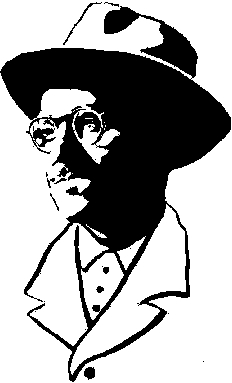
\includegraphics[width=2cm]{03} % 2cm para carta, 1.5cm para medio oficio.
%\end{center}
% \small para carta, \footnotesize para medio oficio.
{\footnotesize\squarepar{\emph{La trascendencia de lo nimio. El humor como poética en los cuentos de Efrén Hernández} de José Julián González Osorno, se terminó de maquetar en Cerrada de Colima núm. 7301, col. Universidades, Heroica Puebla de Zaragoza (México). El manuscrito se capturó con el editor de texto plano \TeX{}maker (5.0.3) y se diagramó en el sistema de composición tipográfico \LaTeX{} desarrollado por Leslie Lamport, basado en el lenguaje de programación \TeX{} creado por Donald E.\,Knuth; el archivo fuente fue compilado mediante el motor de tipografías \hologo{pdfTeX} desarrollado por \hologo{HanTheThanh}. En su composición se empleó tipografía Cochineal, \emph{fork} de Crimson de Sebastian Kosch realizada por Michael Sharpe. Las imágenes se manipularon en \textsc{gimp} (2.10.22); la portada se diseñó en LibreOffice Draw (7.3.0.3). Disposición tipográfica realizada para papel \emph{Bond} tamaño carta de 90\,gr. Diseño y formación:}}
\begin{center}
\small\textcalligra{\href{muxkernel@gmail.com}{Tuxkernel}}
\end{center}
%\begin{center}
%\Bart
%\end{center}
\vfill
% PÁGINA EN BLANCO
\newpage
\pagestyle{empty}
\null\vfill
\end{document}
